This chapter discusses the transient multiphysics simulation results of the
\gls{MSFR} from Moltres for four accident scenarios. These scenarios, adapted
from Fiorina et al.'s work \cite{fiorina_modelling_2014}, include unprotected
instances of reactivity insertion, loss of heat sink, loss of flow, and pump
overspeed accidents. The term ``unprotected'' means no external interventions
occur in these scenarios. As such, these simulations
give an insight on the \gls{MSFR}'s passive safety capabilities in the absence
of any active safety system. This work used the steady-state configuration
presented in the previous chapter as the initial conditions for the transient
simulations discussed in this chapter. Specifically, all steady-state spatial
values for neutron flux, delayed neutron precursor concentration, temperature,
velocity, and pressure were imported as the initial state of the transient
scenarios.

As noted by Fiorina et al. \cite{fiorina_modelling_2014}, explicit decay heat
modeling has a negligible effect in reactivity-, and pump-initiated
transients. Furthermore, only their Polimi model had decay
heat modeling capabilities. Therefore, they presented results from their
Polimi and TUDelft model for the four accident scenarios without decay heat
modeling and enabled decay heat modeling for the loss of heat sink transient
scenario only. This work also ran all transient simulations without the decay
heat model for a fair comparison. The only exception is loss of heat sink
scenario in which two separate simulations with and without the decay heat
model were run. More generally, this work imposed various other simplifying
assumptions in our transient models to match their implementations as closely
as possible, within Moltres' capabilities. The details of the setup for each
transient simulation are in their respective sections.

\section{Unprotected Reactivity Insertion}

Reactivity insertion accidents are a type of nuclear accident caused by
unintended positive
reactivity insertions. The excess reactivity causes the power output and
temperatures in nuclear reactors to rise to potentially dangerous levels. In
\glspl{MSR}, a positive reactivity insertion could occur when the online
refueling system injects excess fissile material into the core. Excessively
high neutron fluences and temperatures negatively impact reactor structural
integrity and increase the risk of containment breach.

This work modeled two unprotected step-wise reactivity insertion scenarios in
Moltres by swapping out the original set of group constant data with two new,
separate sets of data from Serpent corresponding to 50 pcm and 200 pcm
reactivity insertions, respectively. The reactivity of the Serpent \gls{MSFR}
models was increased by increasing the $^{233}$U-to-$^{232}$Th ratio in
the fuel salt.

The focus of this transient study is the neutronic and thermal-hydraulic
behavior of the reactor core. Thus, this work assumes that the heat exchanger
and the associated power generation equipment (generator turbines, heat sinks,
etc.) can withstand all variations in the power output during the transients.

Figures \ref{fig:50pcmheat} and \ref{fig:50pcmtemp} show the power output and
average core temperature increase following the 50 pcm step-wise reactivity
insertion in the Moltres, Polimi, and TUDelft models. The initial prompt
response to the reactivity insertion raises power to 4 GW by $t=0.001$ s.
Figure \ref{fig:50pcmjump} shows the rise in power output specifically during
the prompt response in a separate plot.
Power continues to rise at a slower rate up to 4.63 GW at around $t=0.005$ s,
at which point the negative reactivity from the Doppler effect and salt
expansion becomes greater
than the initial +50 pcm insertion. Power continues to fall as the average
core temperature rises. The slight change in slope occurs at $t=0.3$ s. The
elapsed time approximately corresponds to the average half-life of the two
shortest-lived delayed neutron precursor (DNP) groups ($t_{1/2}=0.195$ s and
$0.424$ s); the decay of the surplus precursors produced in the initial phase
negates a fraction of the negative reactivity from the elevated core
temperature. By $t=3$-$4$ s, most of the heated salt and \glspl{DNP} from the
initial phase will have circulated around the primary loop and returned to the
core. The heated salt causes a small, noticeable dip in power before the power
output stabilises. The core tends to a new equilibrium average temperature
approximately 7.5 K higher than the initial average temperature.

\begin{figure}[htbp!]
    \centering
    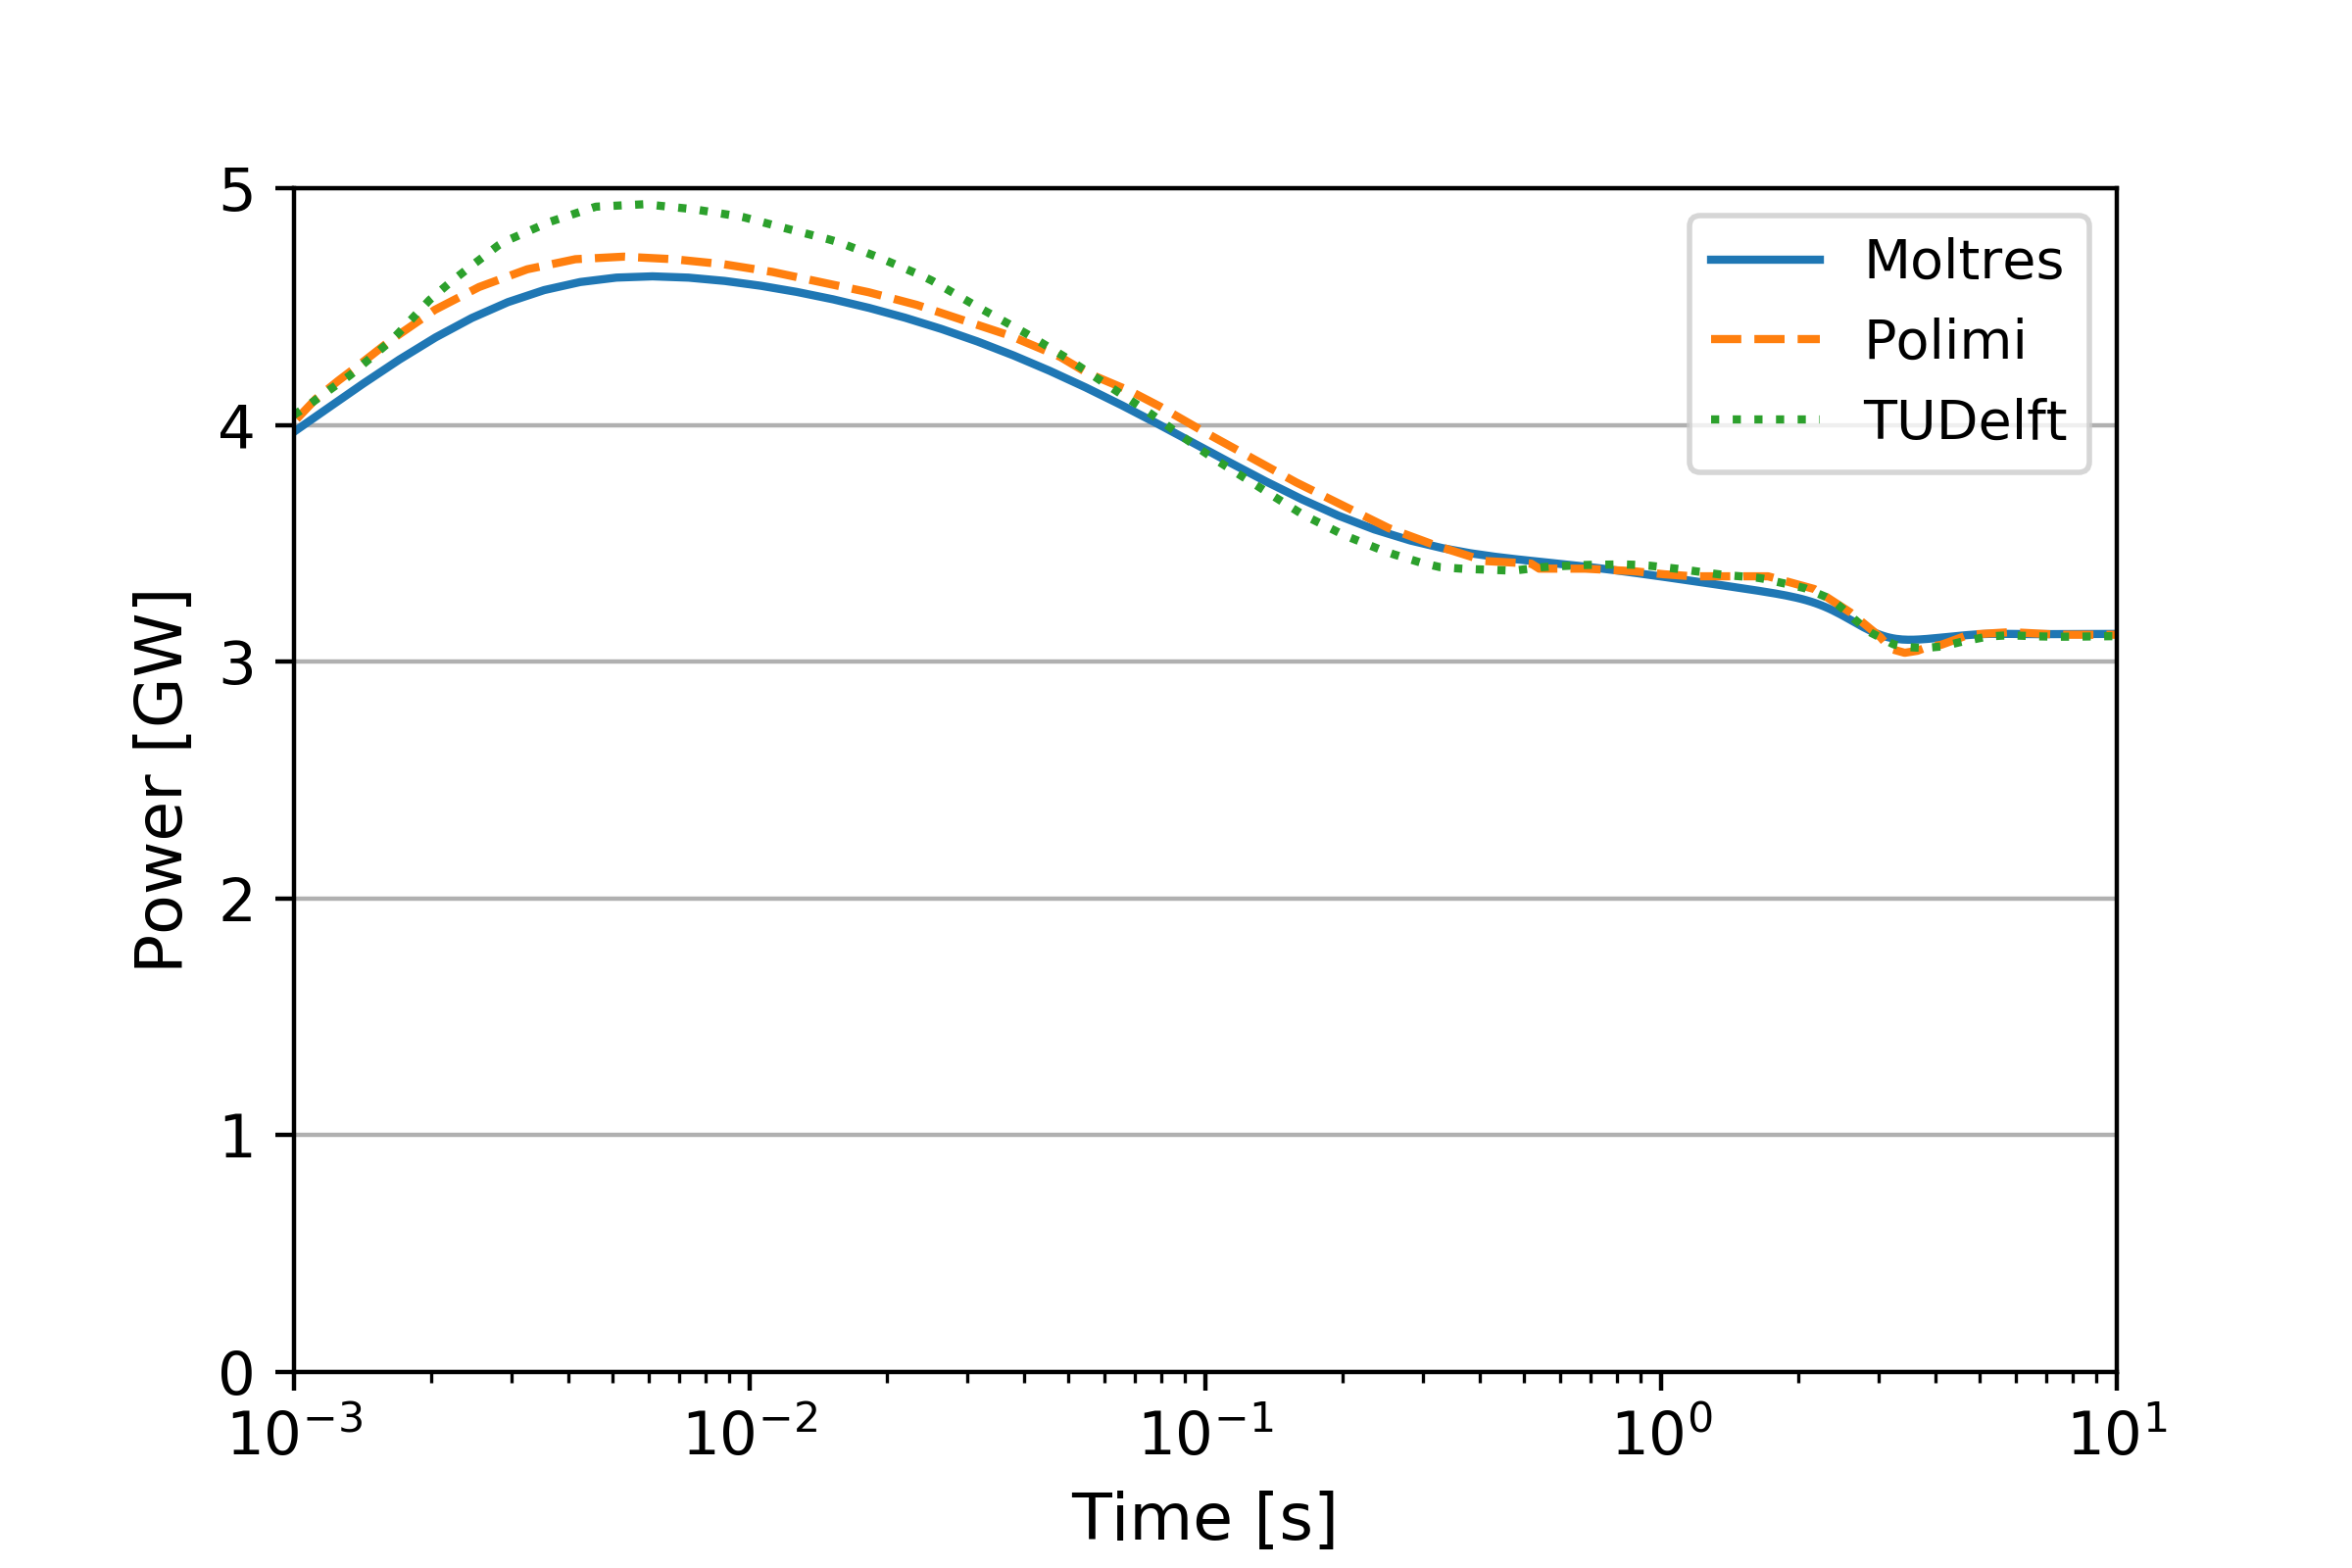
\includegraphics[width=.85\textwidth]{50pcm-heat}
    \caption{Power output following
    a 50 pcm step-wise reactivity insertion in the Moltres, Polimi, and
    TUDelft models \cite{fiorina_modelling_2014}.}
    \label{fig:50pcmheat}
%
    \centering
    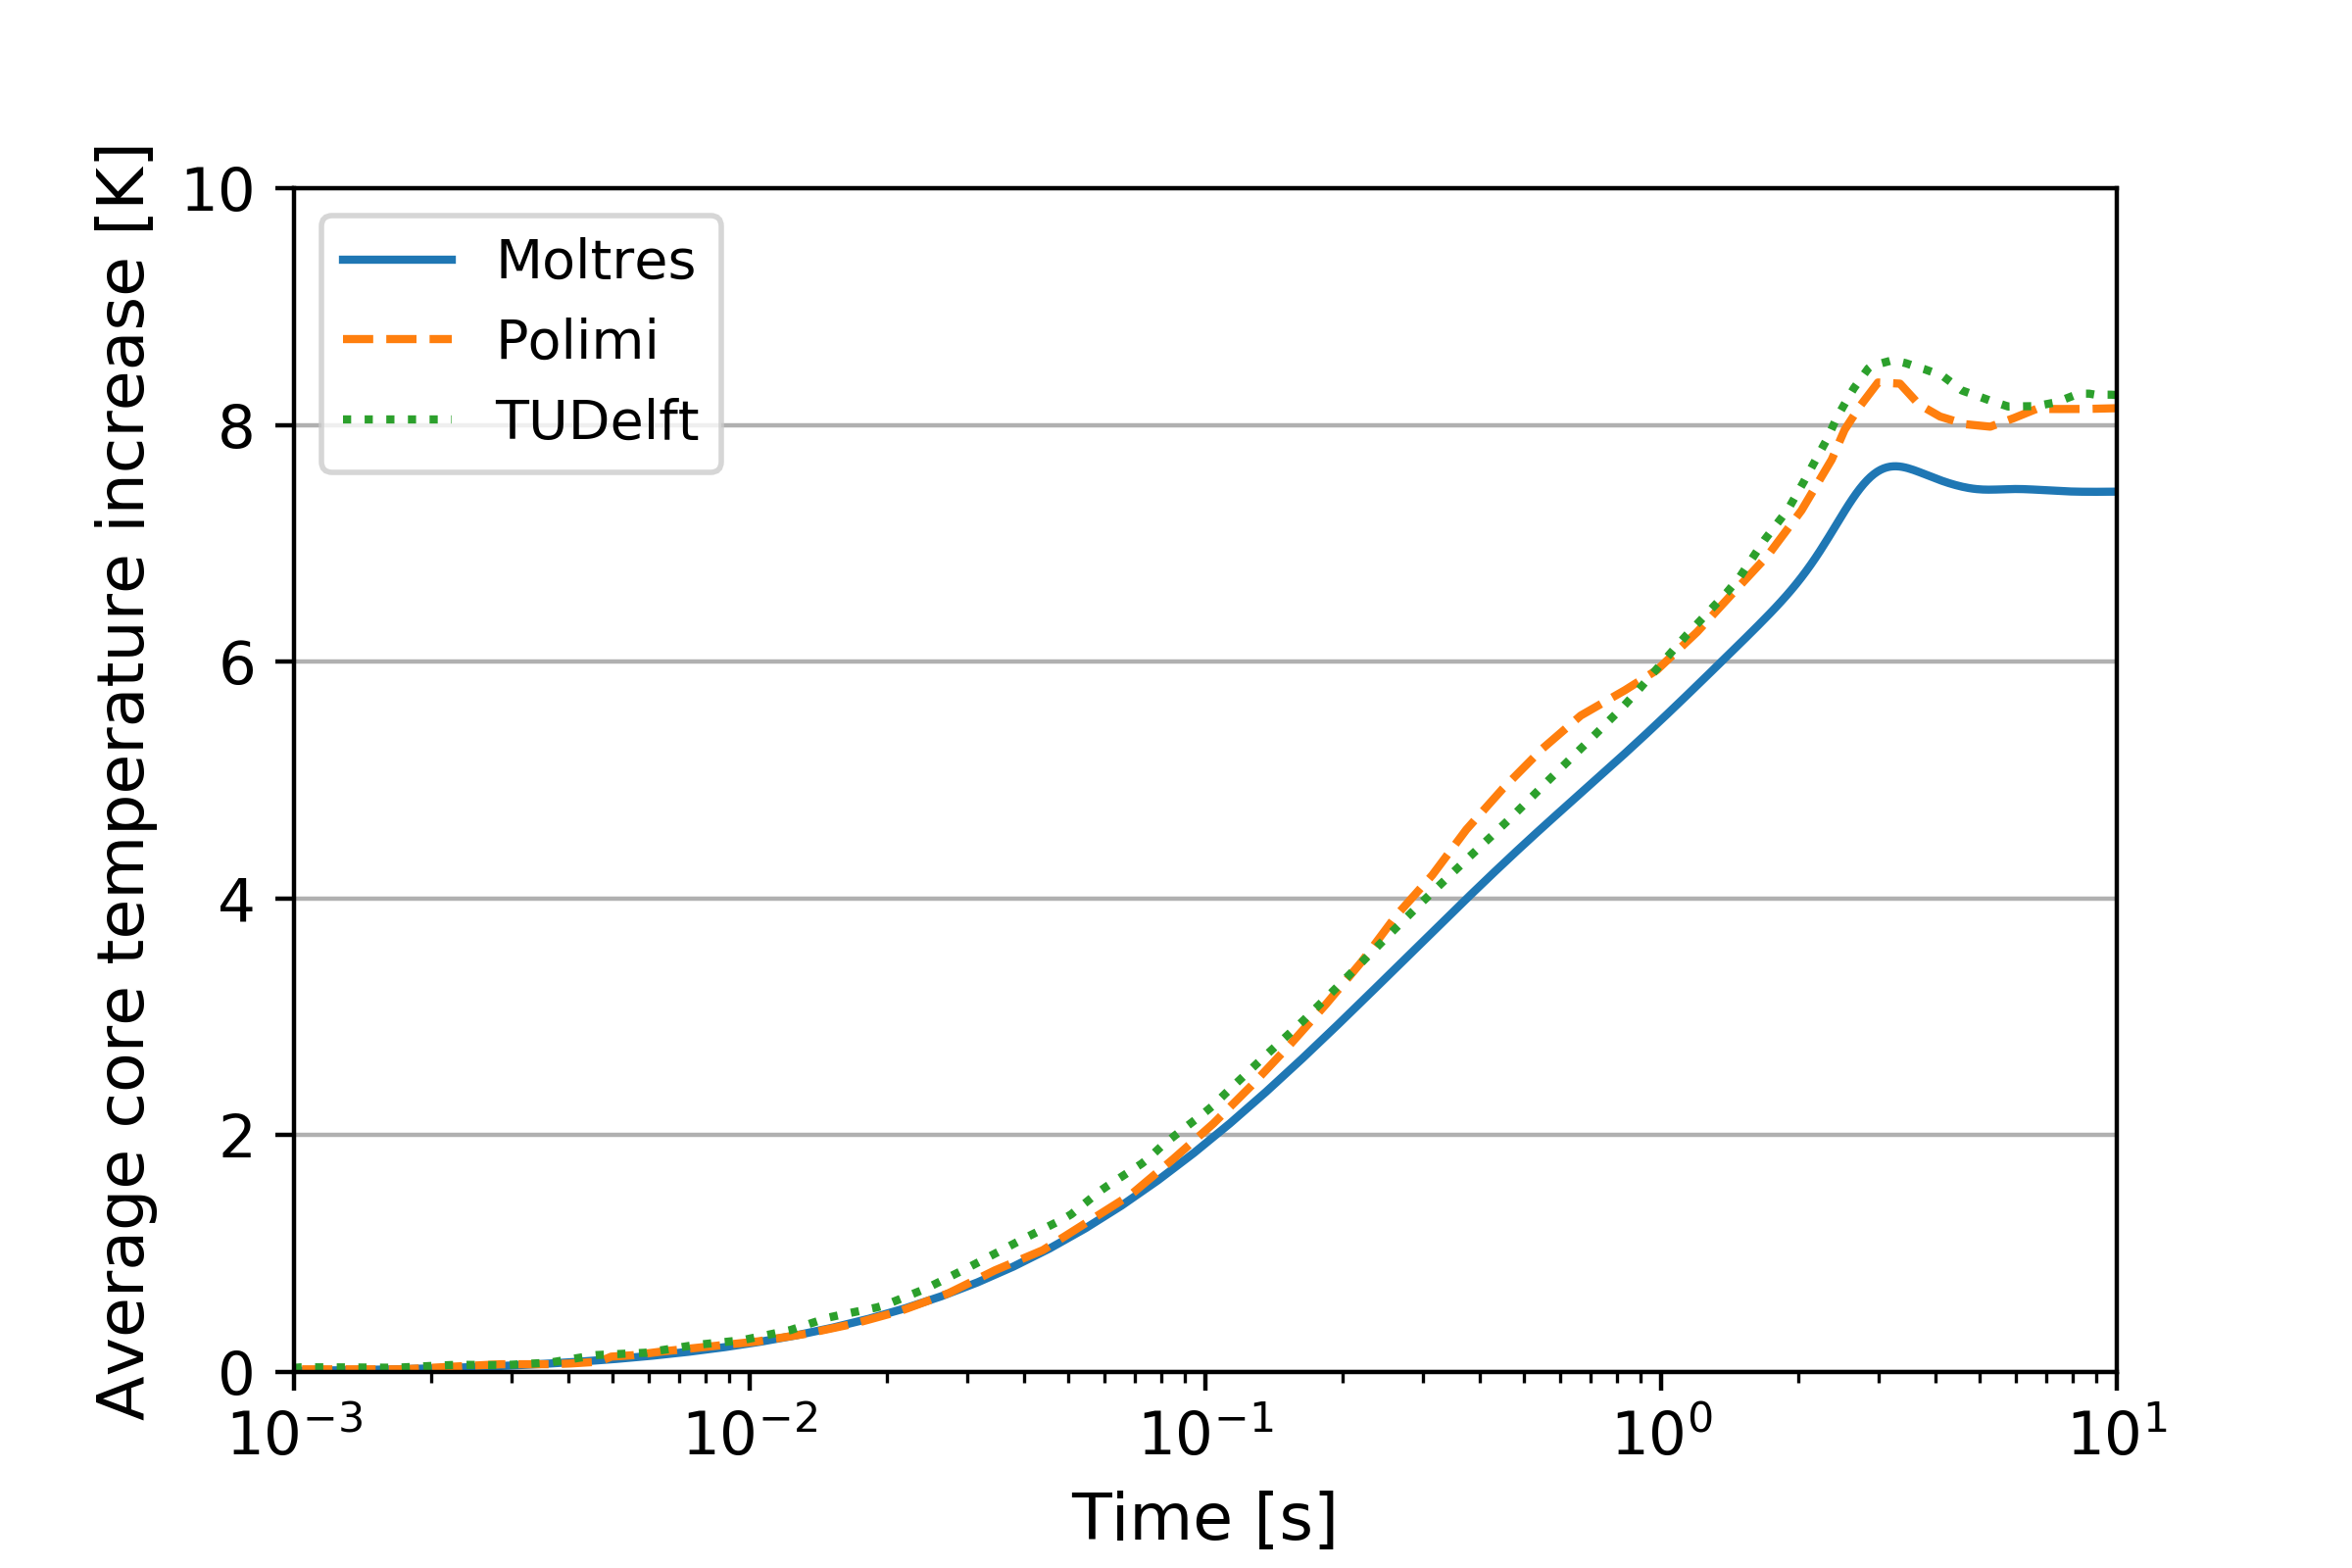
\includegraphics[width=.85\textwidth]{50pcm-temp}
    \caption{Average core temperature increase following
    a 50 pcm step-wise reactivity insertion in the Moltres, Polimi, and
    TUDelft models \cite{fiorina_modelling_2014}.}
    \label{fig:50pcmtemp}
\end{figure}

\begin{figure}[htbp!]
    \centering
    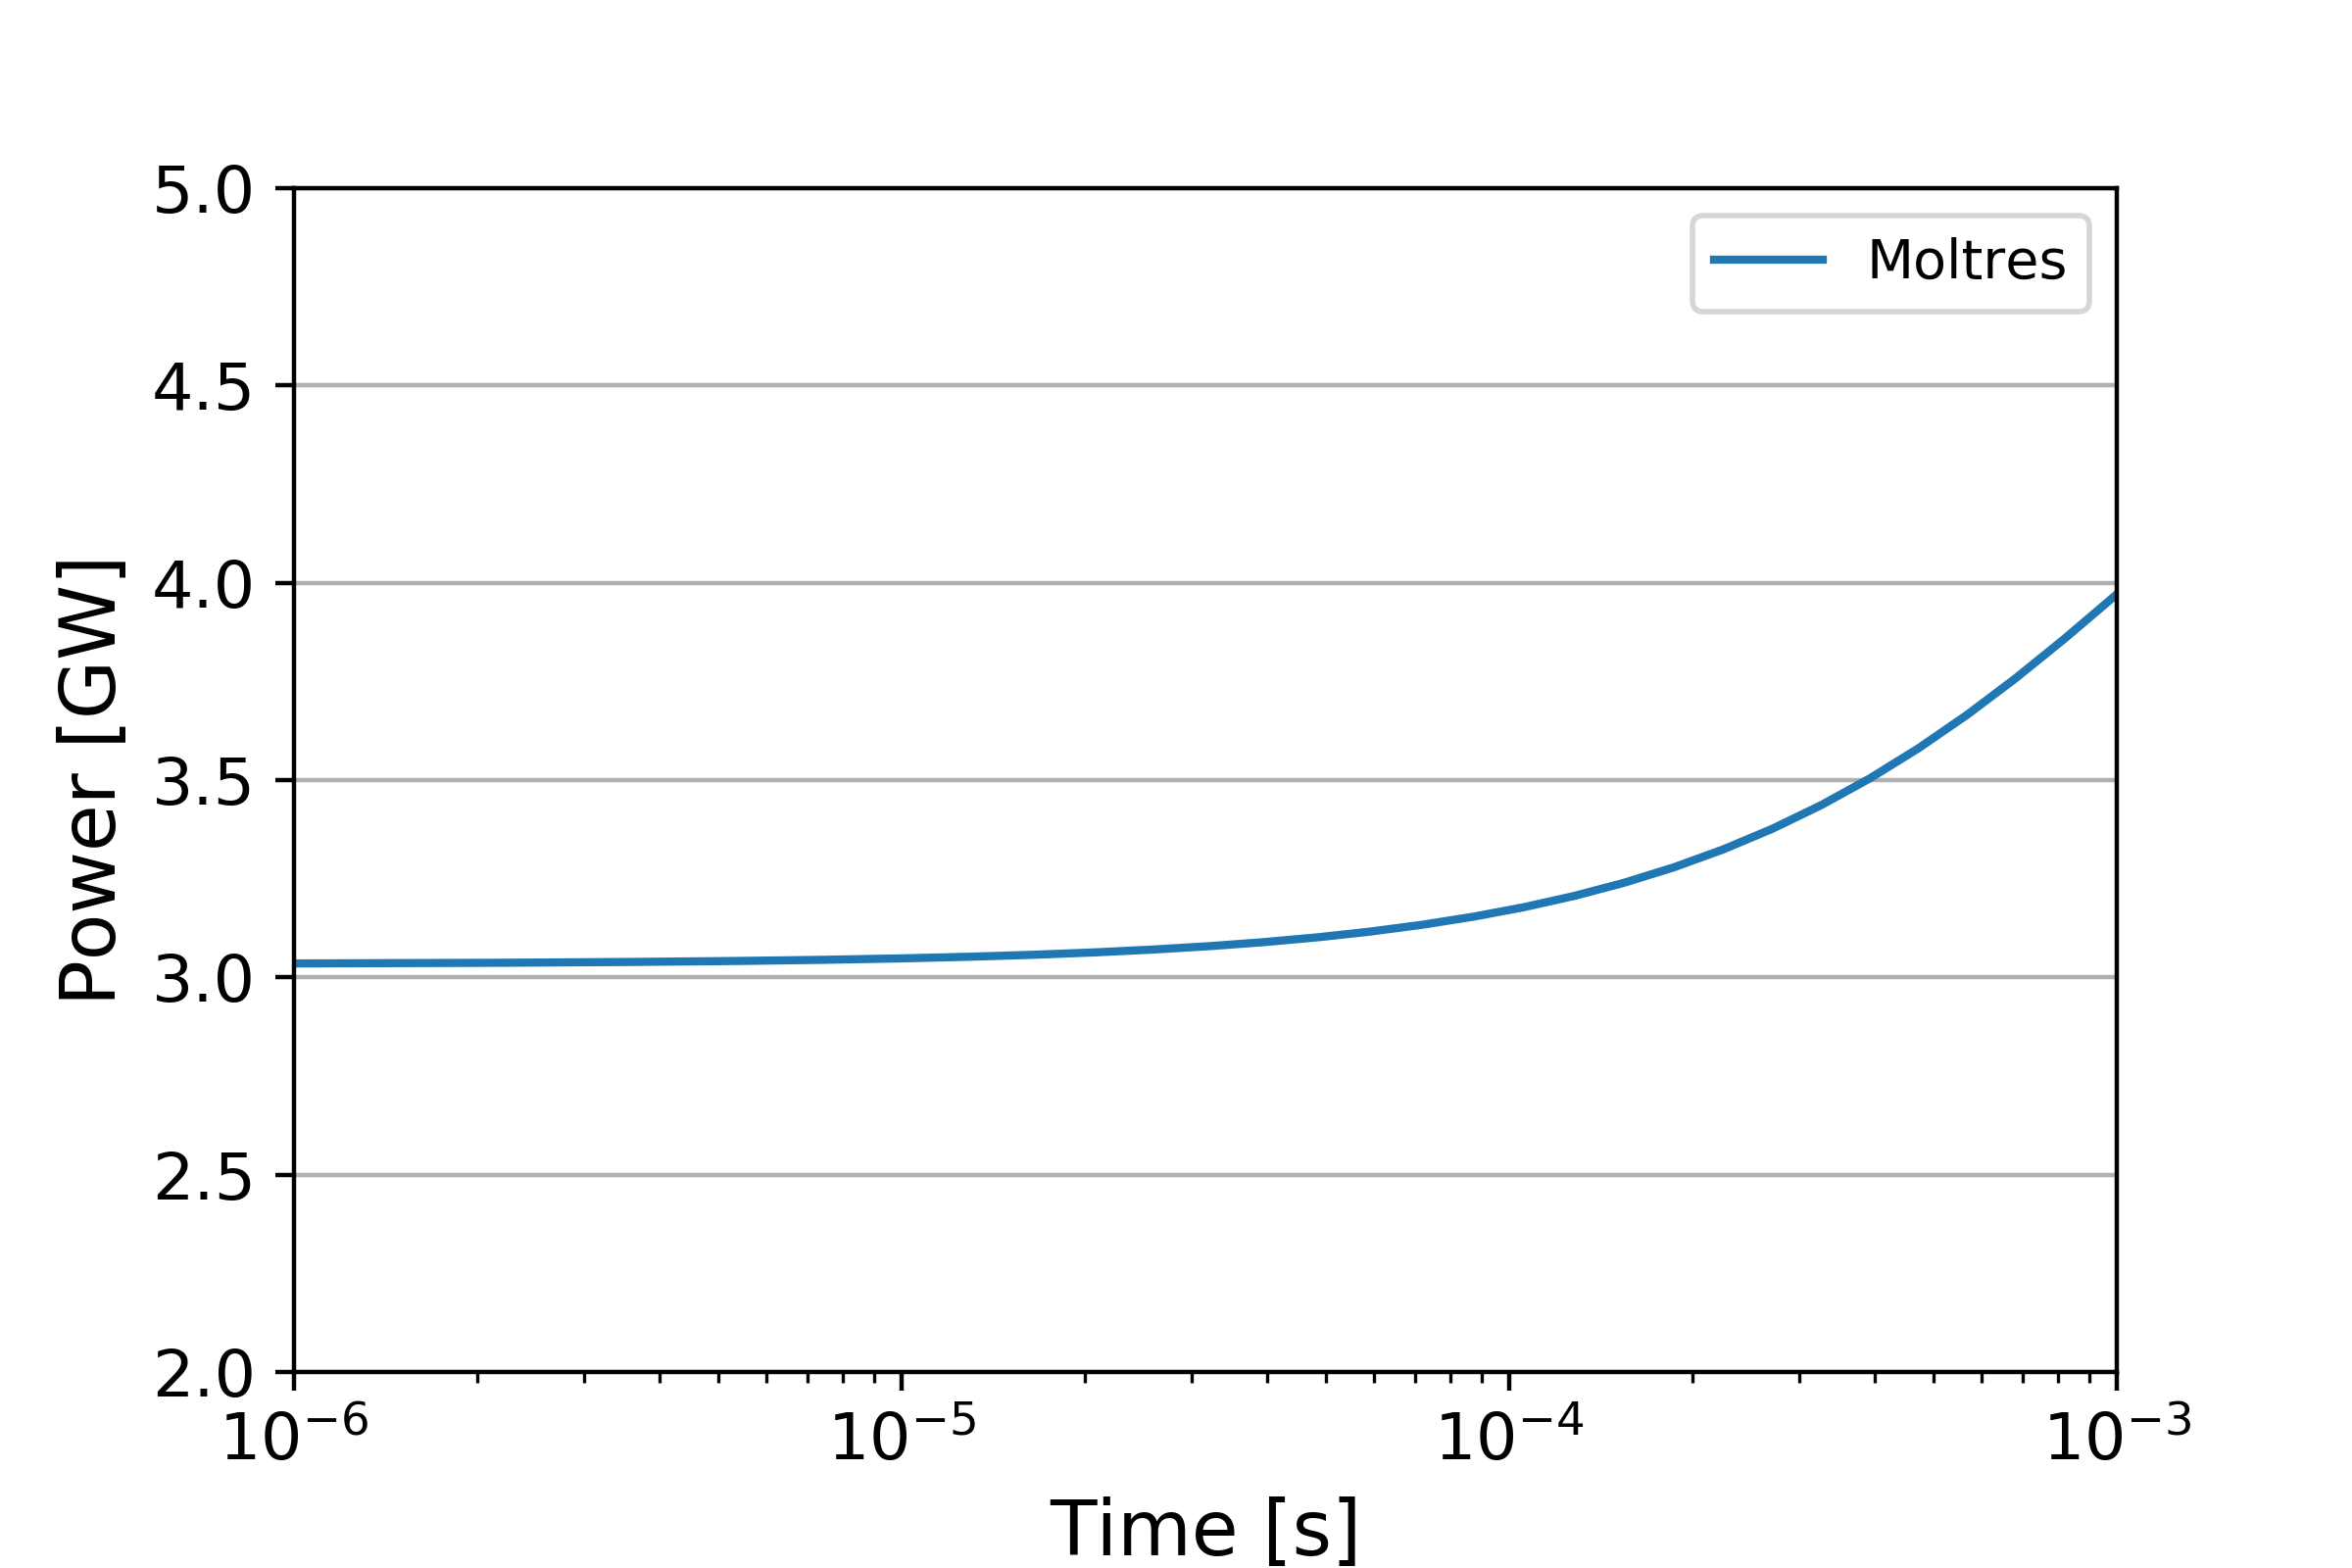
\includegraphics[width=.7\textwidth]{50pcm-jump}
    \caption{Power output during the prompt response following
    a 50 pcm step-wise reactivity insertion in the Moltres, Polimi, and
    TUDelft models \cite{fiorina_modelling_2014}.}
    \label{fig:50pcmjump}
\end{figure}

The results from Moltres show good agreement with the results from the Polimi
and TUDelft models; Moltres reproduced all of the individual features in both
plots. The magnitude of the reactor response is the most significant
difference. Moltres predicts a smaller peak in the power output and a smaller
overall increase in the average core temperature mainly due to the
more negative temperature reactivity coefficient in Moltres than in the Polimi
and TUDelft models. The temperature reactivity coefficient $\alpha_T$ in
Moltres is $-7.184$ pcm K$^{-1}$ (Table \ref{table:alpha}), as opposed to
approximately $-6.5$ pcm K$^{-1}$ within the relevant temperature range in the
Polimi and TUDelft models. Therefore, the results show a smaller temperature
increase in the Moltres model for the same reactivity insertion. Multiplying
the average
core temperature increase at $t=10$ s with $\alpha_T$ gives us $-7.184$ pcm
K$^{-1} \times 7.46$ K $= -53.6$ pcm, which is approximately equal to the 50
pcm reactivity insertion.

\begin{figure}[htbp!]
    \centering
    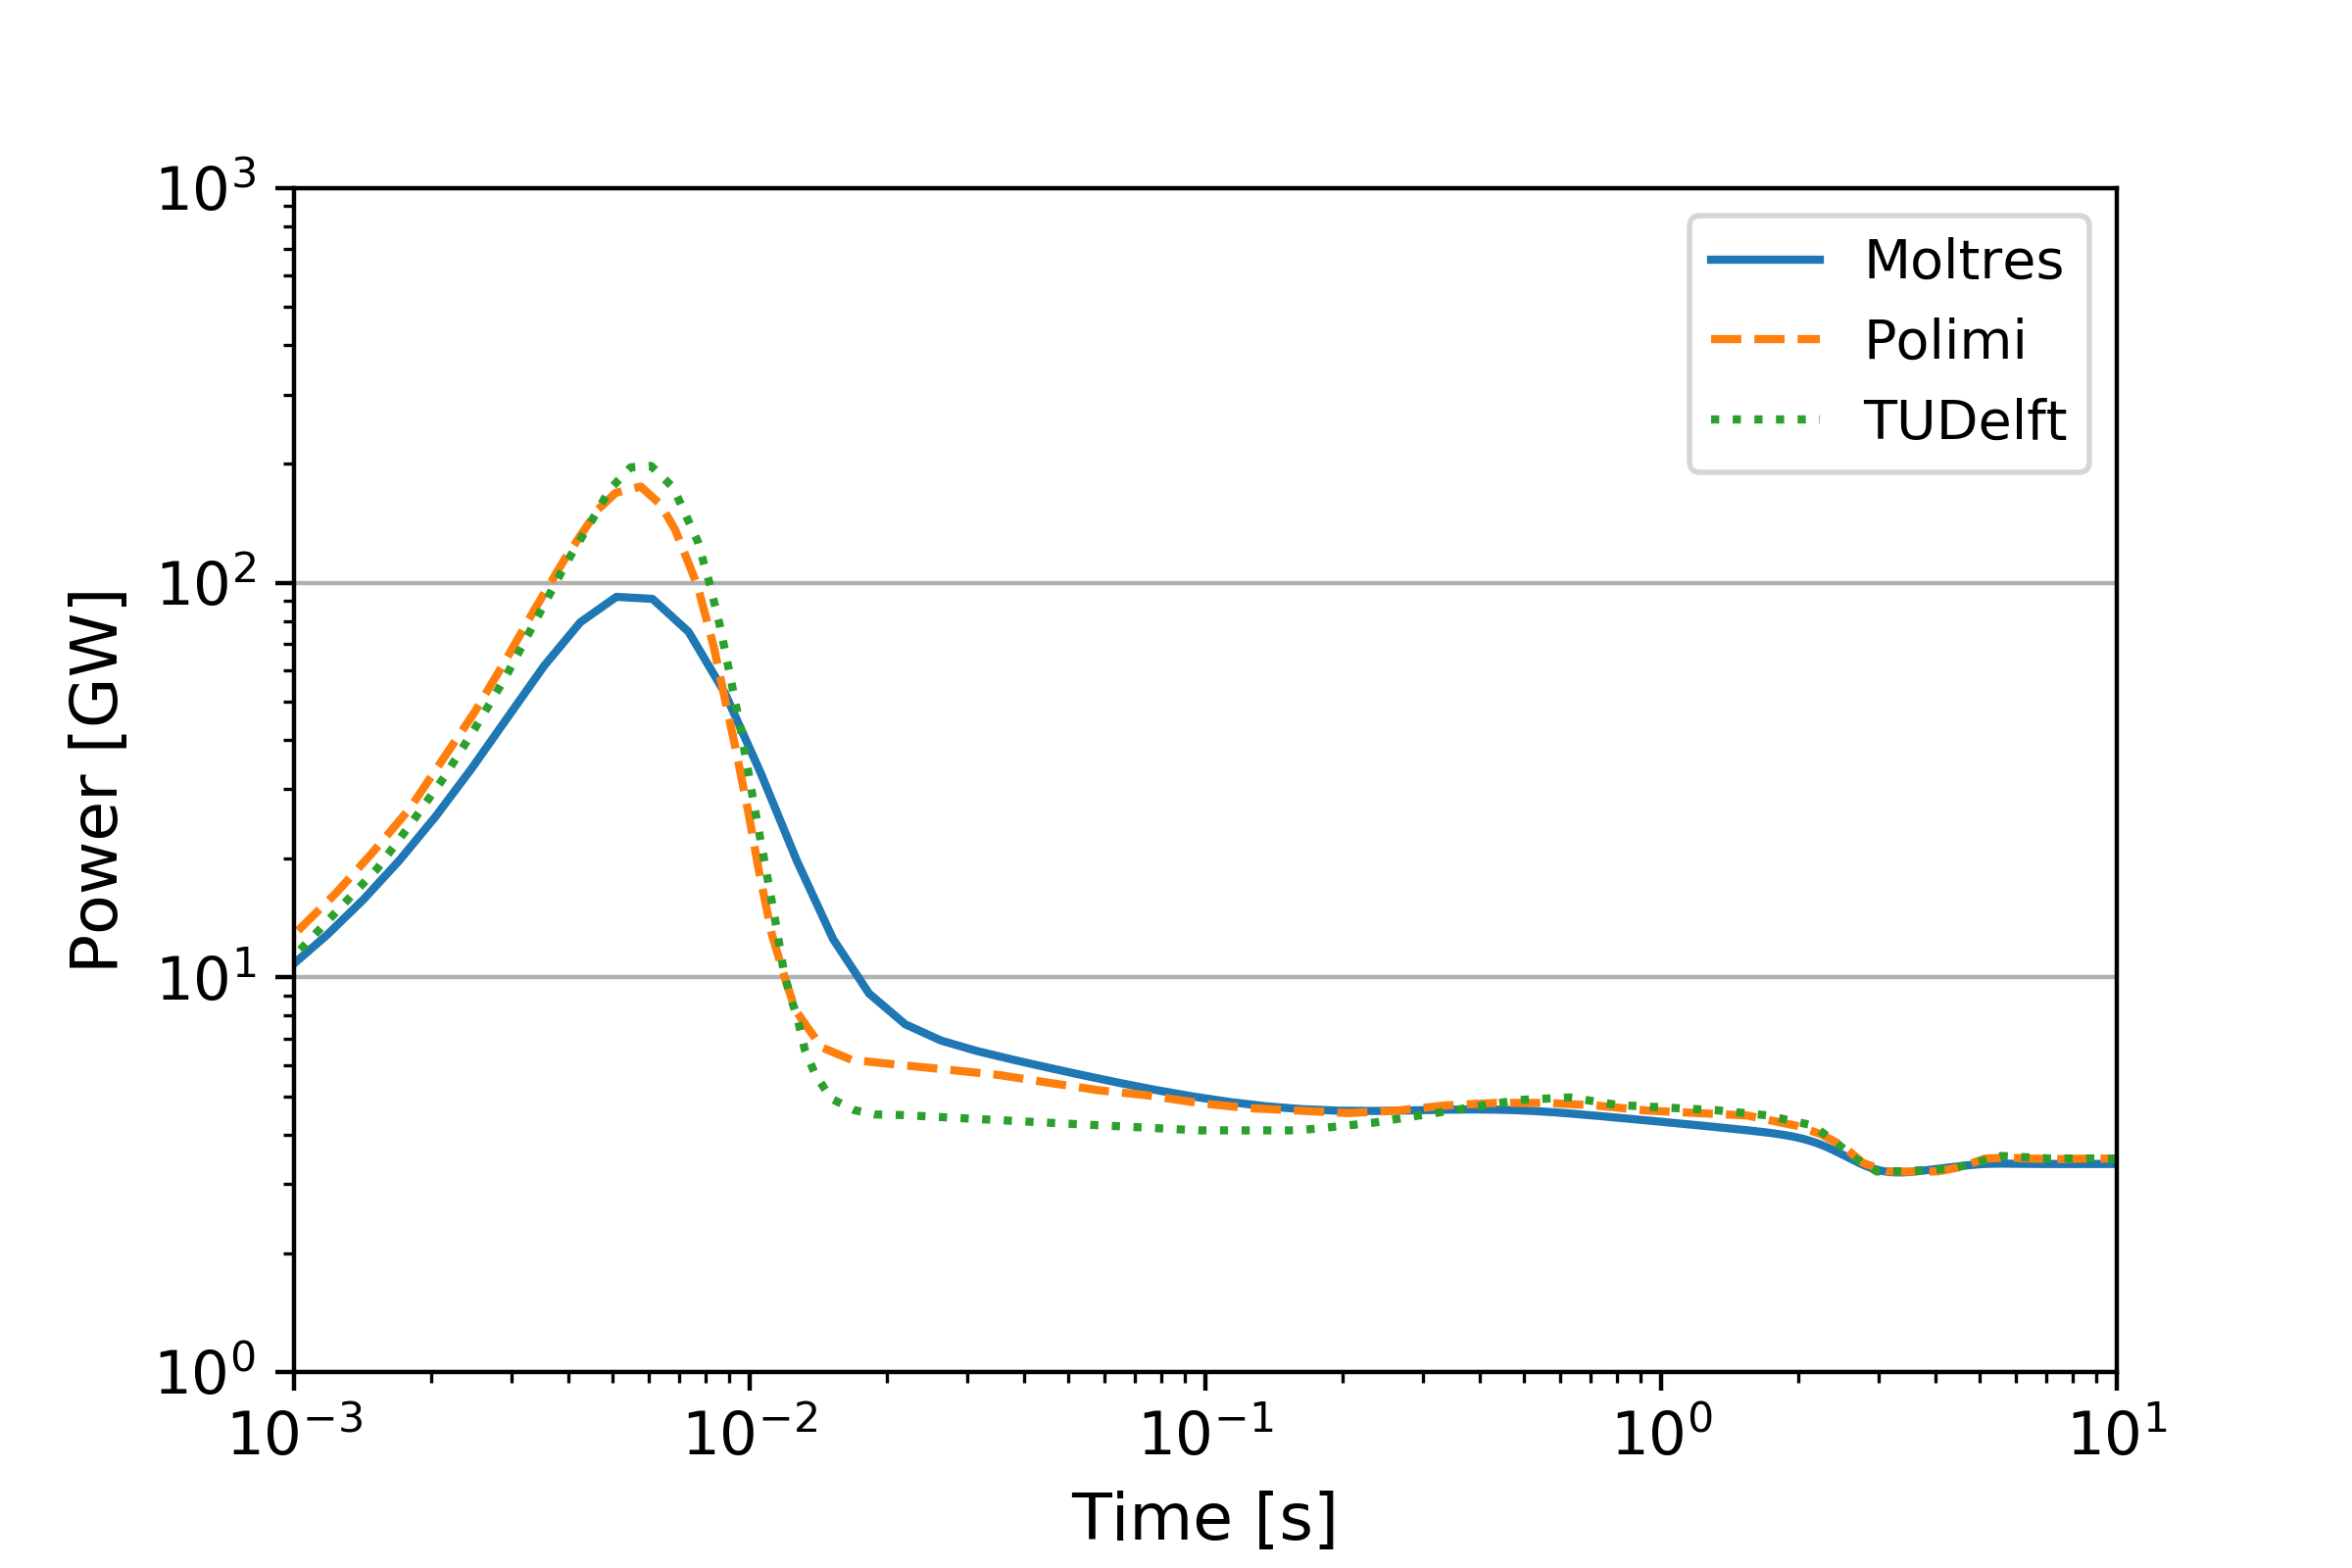
\includegraphics[width=.85\textwidth]{200pcm-heat}
    \caption{Power output following
    a 200 pcm step-wise reactivity insertion in the Moltres, Polimi, and
    TUDelft models \cite{fiorina_modelling_2014}.}
    \label{fig:200pcmheat}
%
    \centering
    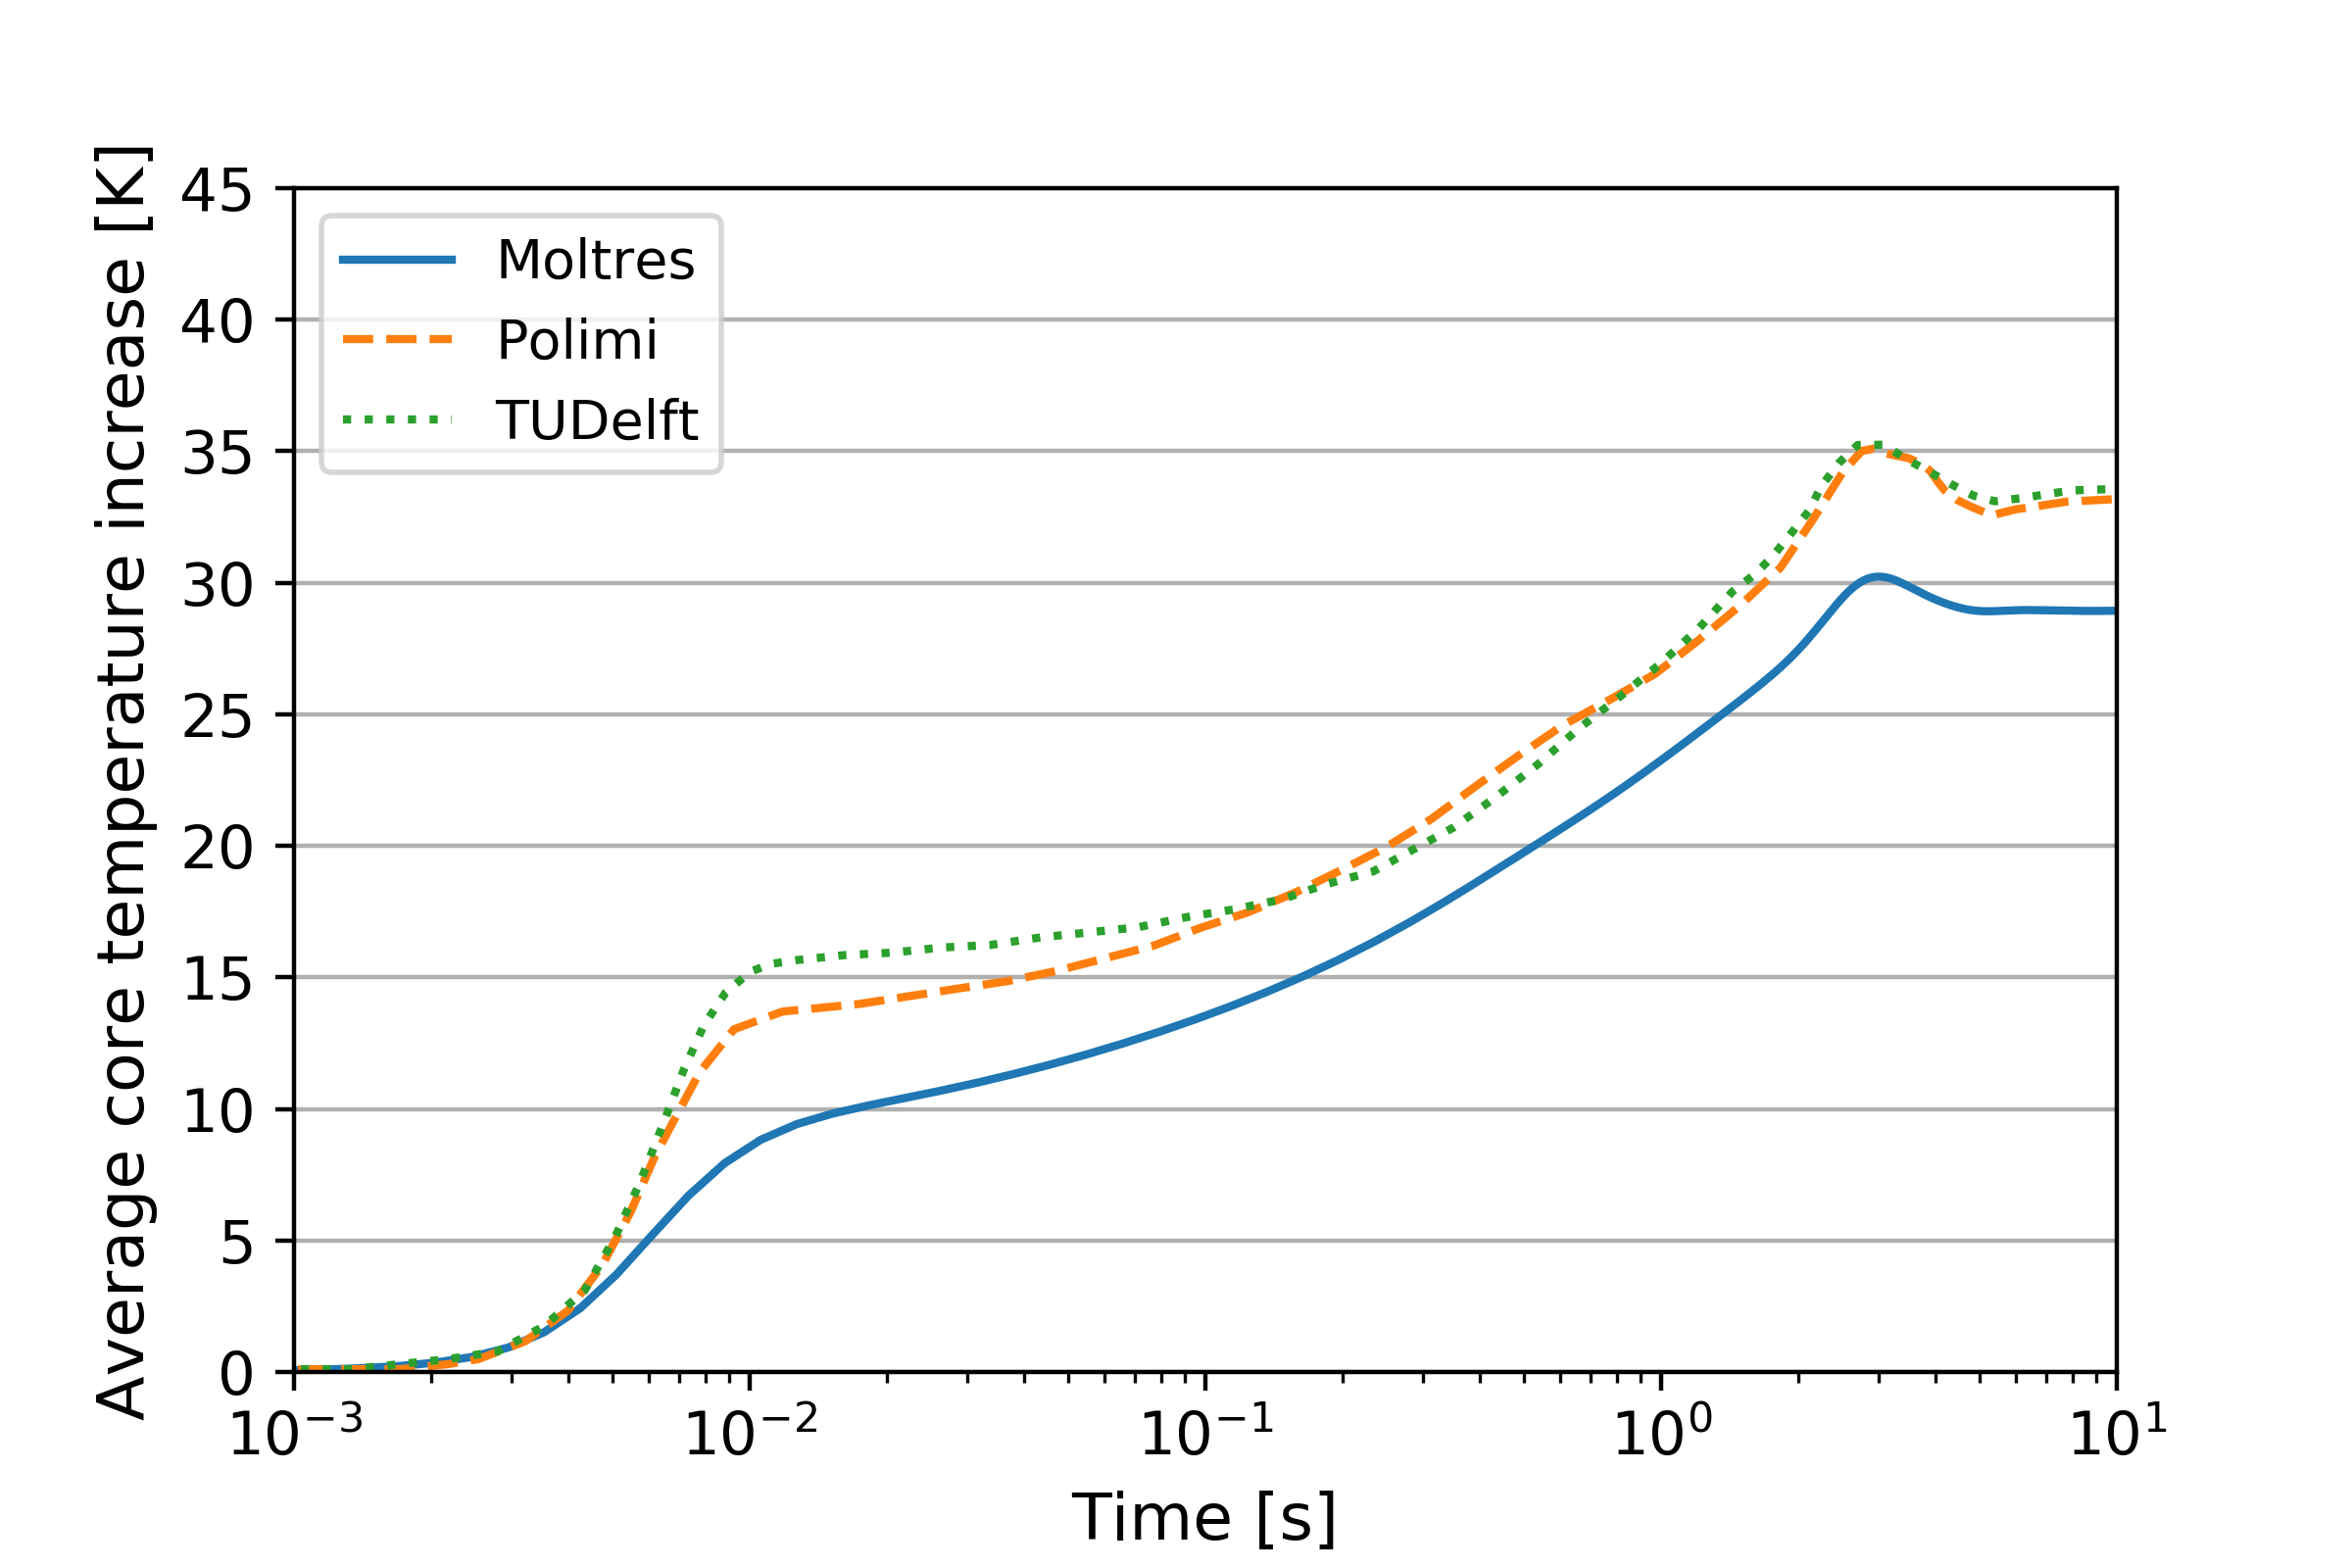
\includegraphics[width=.85\textwidth]{200pcm-temp}
    \caption{Average core temperature increase following
    a 200 pcm step-wise reactivity insertion in the Moltres, Polimi, and
    TUDelft models \cite{fiorina_modelling_2014}.}
    \label{fig:200pcmtemp}
\end{figure}

The results for the 200 pcm reactivity insertion scenario show similar trends
to the 50 pcm case. The greater reactivity insertion elicits a stronger
prompt response in the power output which peaks at 92.1 GW. The average core
temperature increases much more rapidly and subsequently triggers a sharper
drop in power output. This results in the clearer distinction in the rate of
core temperature increase before and after $t=0.01$ s. In this transient, we
also observe greater deviation between Moltres and the other models arising
from the differences in the temperature reactivity coefficients. Overall,
Moltres' results show good agreement with the Polimi and TUDelft results.
The differences arise mainly due to the differences in the temperature
reactivity coefficients.

\section{Unprotected Loss of Heat Sink}

An unprotected loss of heat sink accident can occur when the pumps in the
intermediate loop fail. The heat exchangers would then lose most of their
cooling capabilities. This work followed Fiorina et al.'s approach in assuming
that the cooling from the heat exchangers decreases exponentially with a time
constant of 1 s and all other parameters held constant
\cite{fiorina_modelling_2014}. As mentioned in the Chapter \ref{chap:ss}, we
will present two sets of results for this transient: 1) without decay heat
modeling, and 2) with decay heat modeling.

\subsection{Without Decay Heat} \label{sec:wodecayheat}

Figures \ref{fig:lohsheat} and \ref{fig:lohstemp} show the power output and
average core temperature increase during the unprotected loss of heat sink
transient in the Moltres, Polimi, and TUDelft models without decay heat
modeling. The power output and average core temperature show little change in
the first two seconds as it takes approximately that amount of time for the
partially cooled salt to migrate to the center of the core. At $t=2$ s, we
observe a sharp spike in average core temperature and a corresponding drop
in power output. The presence of delayed neutron precursors (DNPs) from the
steady-state operating conditions momentarily halt the increase in temperature
at around $t=5$ s. The average core temperature continues to rise while the
power output falls through the rest of the transient.

The results from Moltres show good agreement with the results from the Polimi
and TUDelft. Moltres reproduced all of the trends in the Polimi
and TUDelft models. The temporary halt in the temperature increase occurs at
a lower average core temperature for Moltres than the other two models. This
is likely due to the difference in the temperature reactivity coefficient
discussed in the reactivity insertion results; a smaller increase in
the average core temperature produces the same decrease in power output.

\begin{figure}[htbp!]
    \centering
    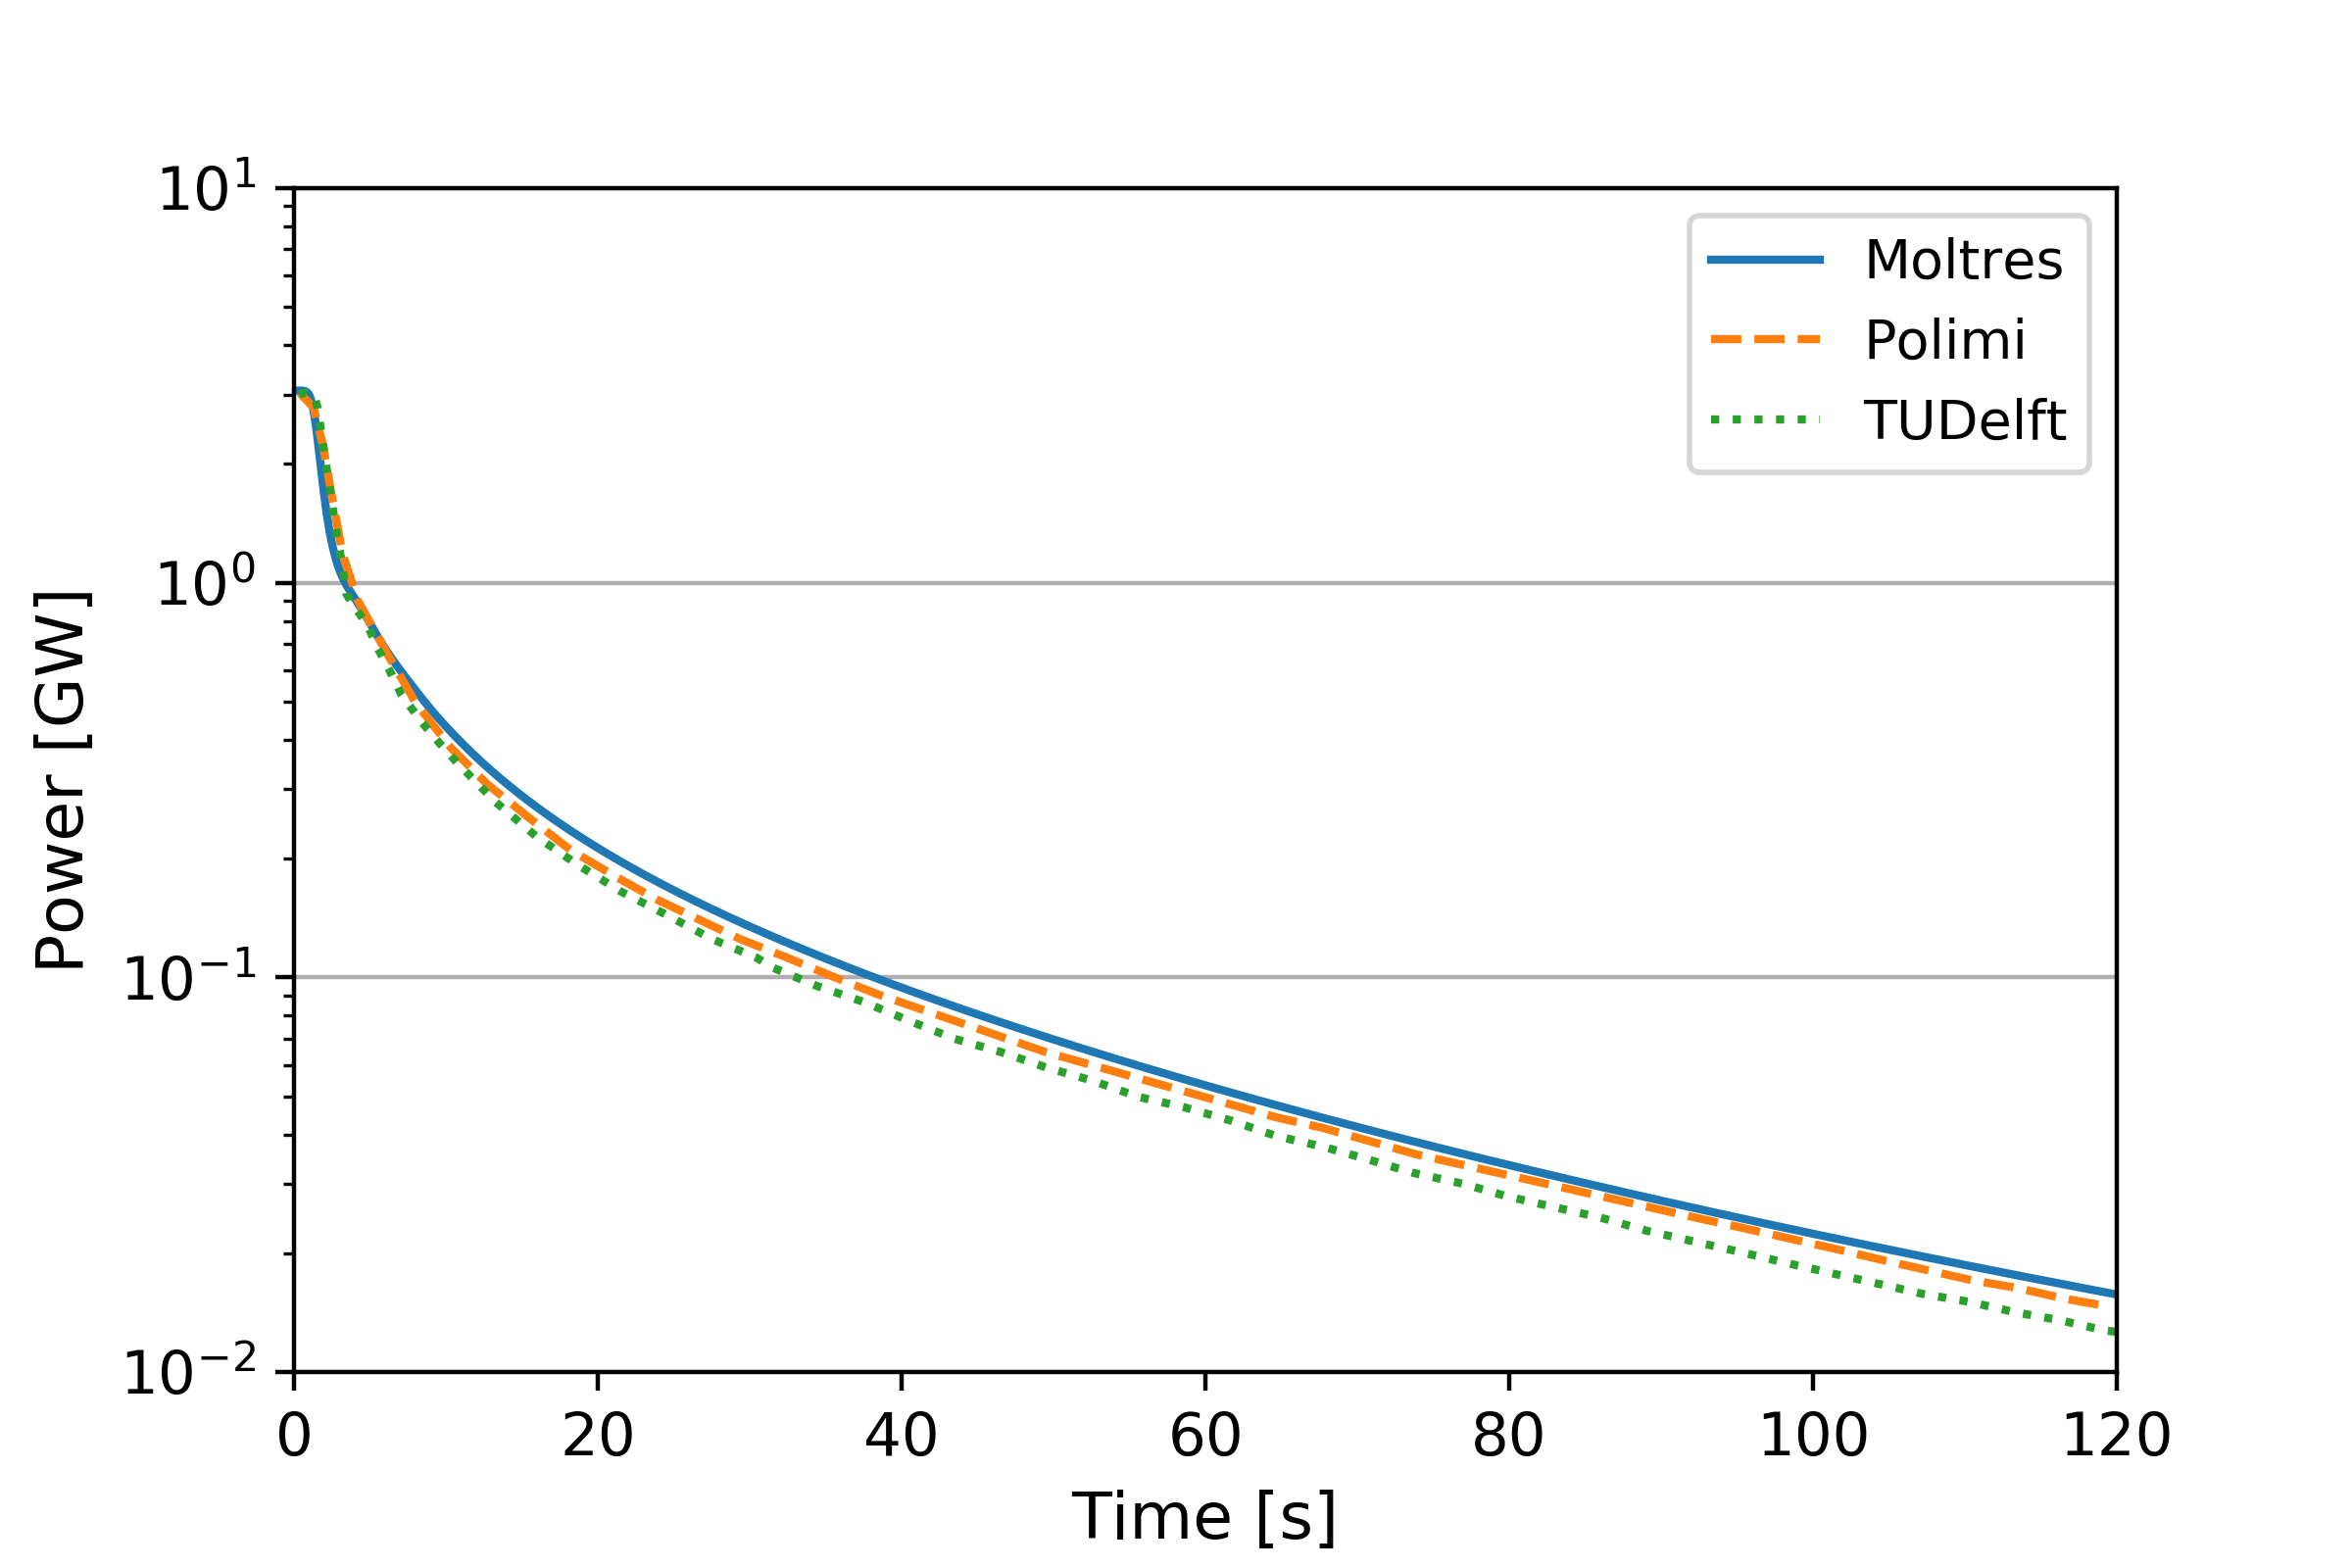
\includegraphics[width=.85\textwidth]{lohs-heat}
    \caption{Power output during
    an unprotected loss of heat sink transient in the Moltres, Polimi, and
    TUDelft models \cite{fiorina_modelling_2014} without decay heat.}
    \label{fig:lohsheat}
    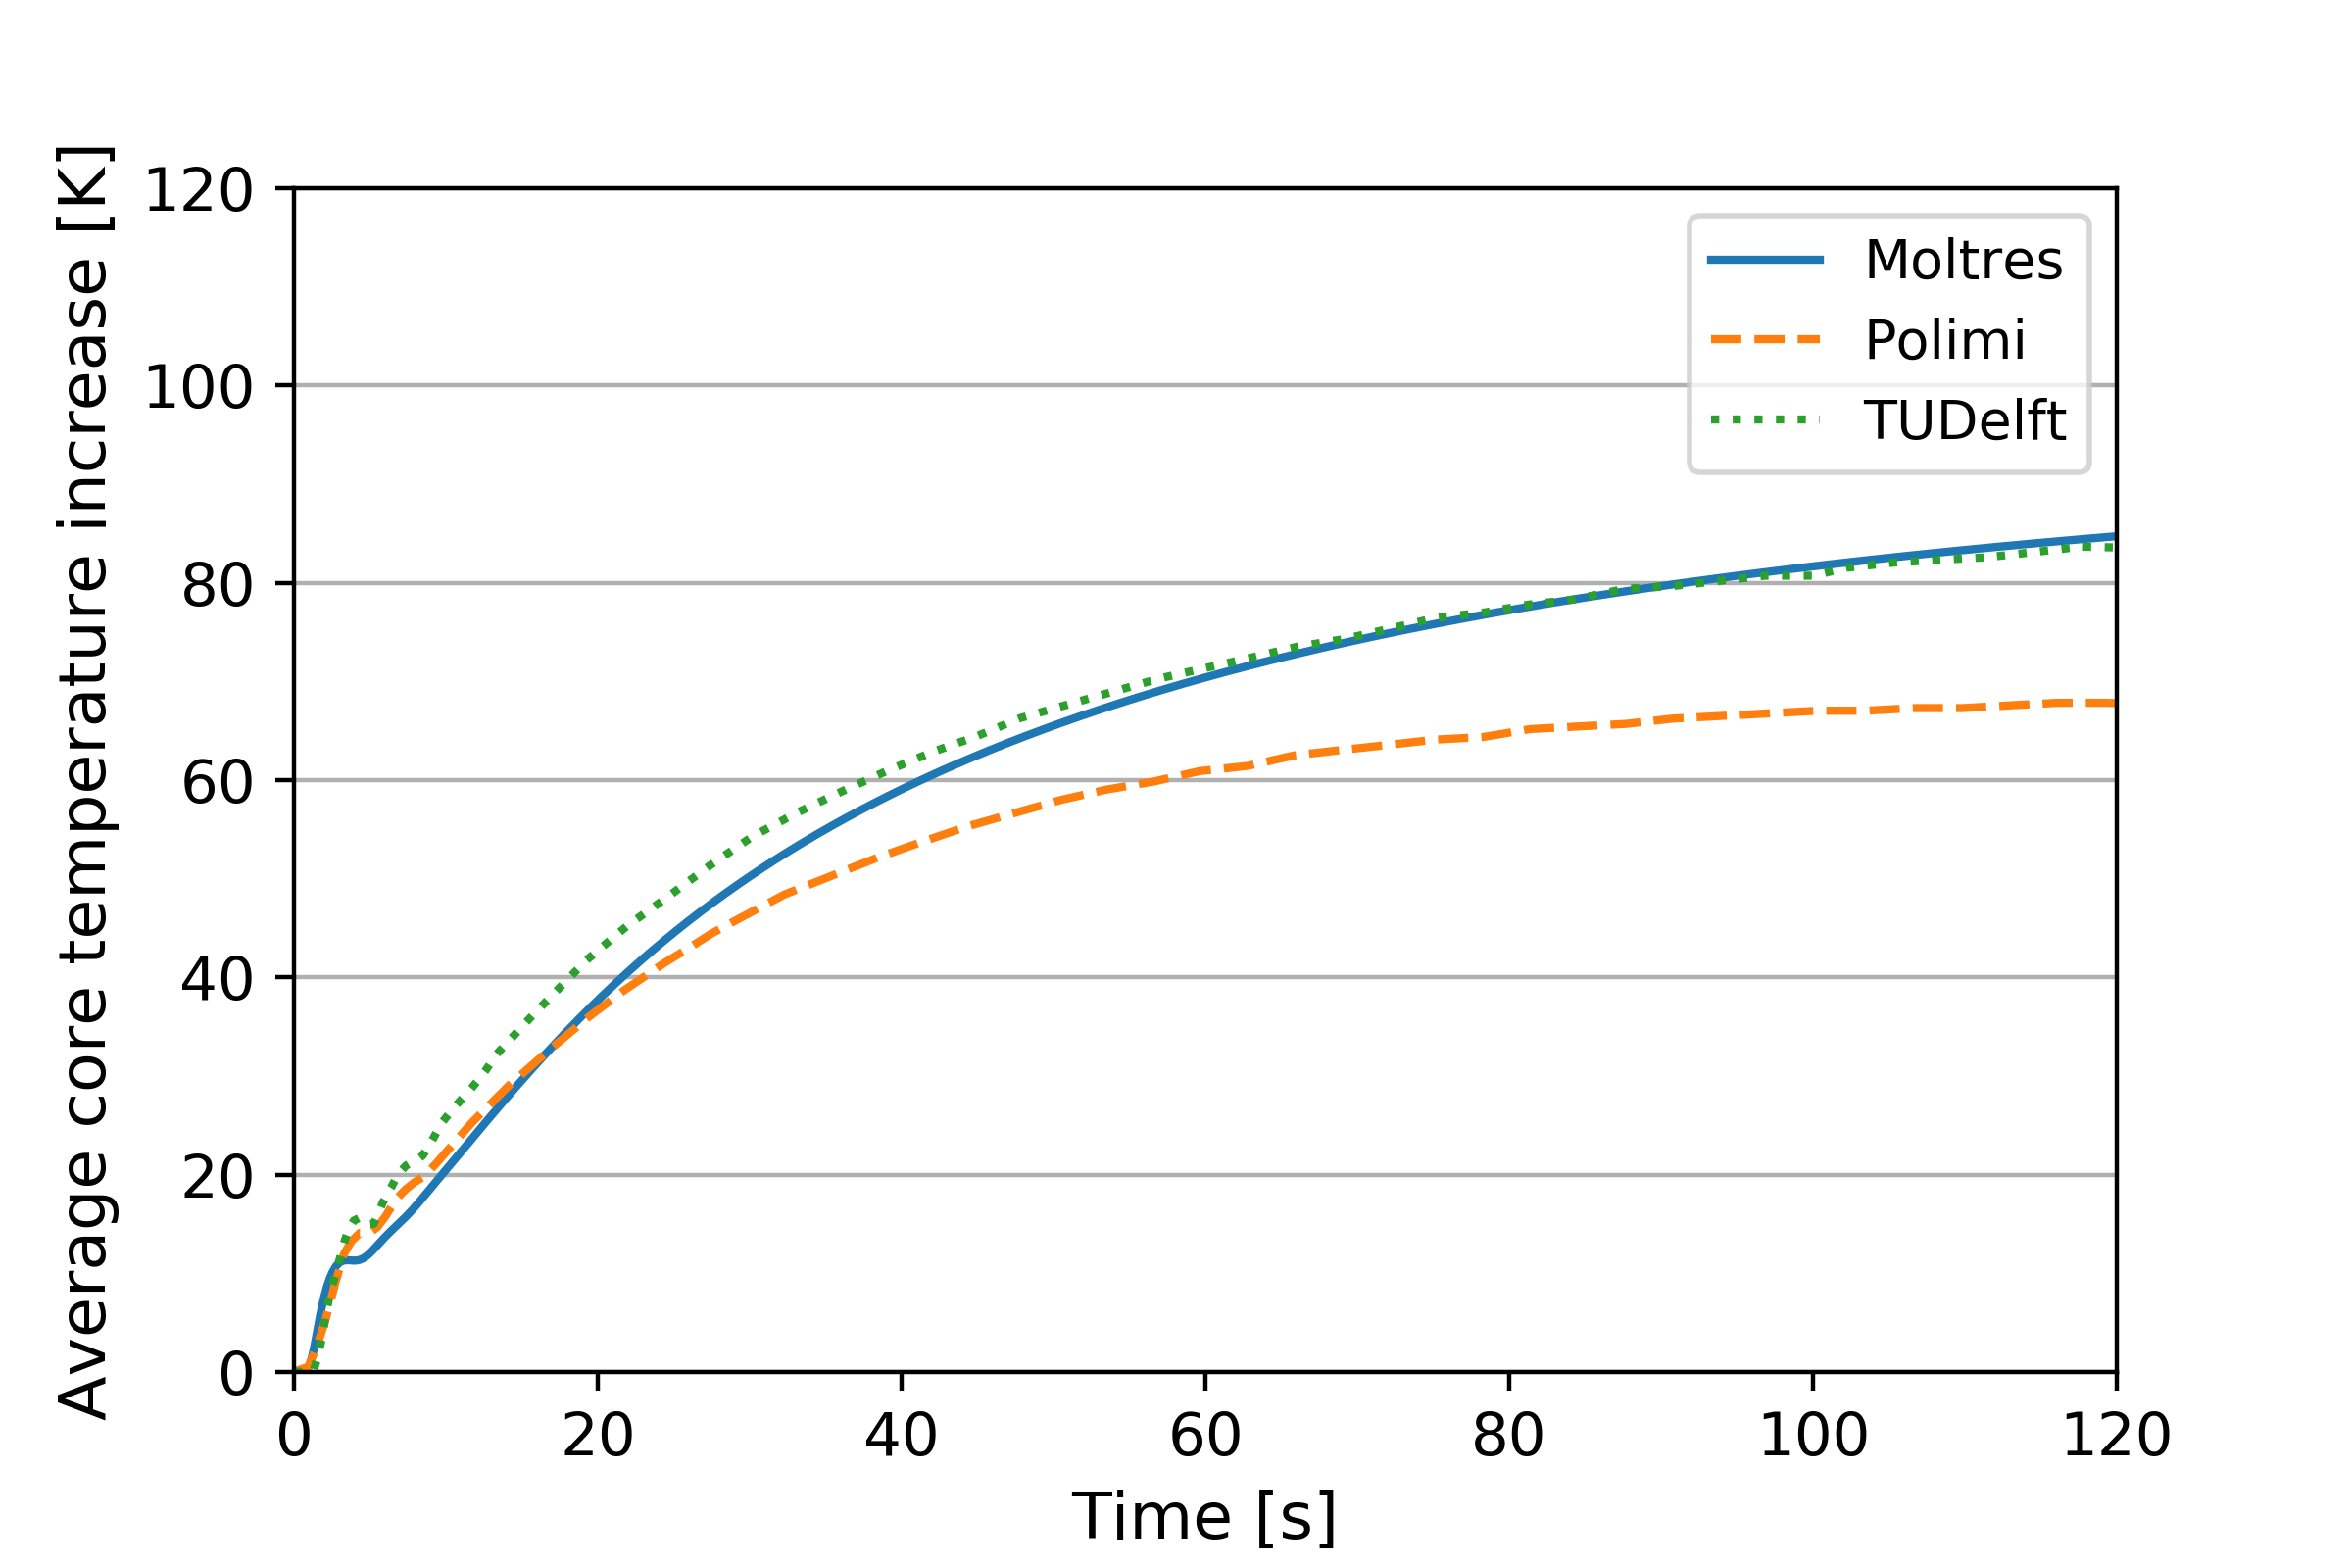
\includegraphics[width=.85\textwidth]{lohs-temp}
    \caption{Average core temperature increase during
    an unprotected loss of heat sink transient in the Moltres, Polimi, and
    TUDelft models \cite{fiorina_modelling_2014} without decay heat.}
    \label{fig:lohstemp}
\end{figure}

\clearpage

\subsection{With Decay Heat}

Decay heat from fission products poses a great safety risk in a loss of
heat sink accident. Section \ref{sec:wodecayheat} showed that prompt fission
power output quickly falls as core temperatures rise. However, decay power
output is independent of the instantaneous neutron flux. Figure
\ref{fig:moltresdecaypower} shows that the decay power output remains
relatively high during a short-term transient. Decay heat becomes the dominant
heat source from $t=34$ s and falls at a much slower rate than prompt heat.
Figure \ref{fig:moltresdecaytemp} highlights the
greater core temperature increase attributed to decay heat as compared with
the results without decay heat. By $t=120$ s, the model with decay heat
records an average core temperature increase that is 45 K higher than the
model without decay heat. The average core temperature reaches approximately
1220 K and would continue to rise further. This places undue thermal stress
and accelerate corrosion rates in the Hastelloy structural material. In the
absence of an auxiliary heat removal system in the primary loop, reactor
operators would have to rely on the freeze plug to drain the core into a drain
tank with emergency cooling systems to keep the salt cool.

Figure \ref{fig:polimidecaytemp} shows the loop-averaged temperature
increase in the Moltres and Polimi models \cite{fiorina_modelling_2014}. The
TUDelft model does not have a decay heat modeling capability. The Moltres
model predicts the same increasing trend in the temperature. The loop-averaged
temperature rises significantly at the start of the transient and continues to
rise at a decreasing rate. The loop-averaged temperature increase in the
Moltres model at $t=120$ s is approximately 17 K lower than that in the Polimi
model. It is difficult to ascertain the exact cause for this difference
without the power profile from the Polimi model with decay heat to compare
with. However, if the decay power output are similar, the stronger negative
temperature reactivity coefficient would cause the prompt power output in the
Moltres model to fall faster than the Polimi model. Consequently, the
loop-averaged temperature would be lower as shown in the figure. Overall, the
results for the loss of heat sink transient agree with the Polimi and TUDelft
model results in both cases, with and without decay heat modeling.

\begin{figure}[htbp!]
    \centering
    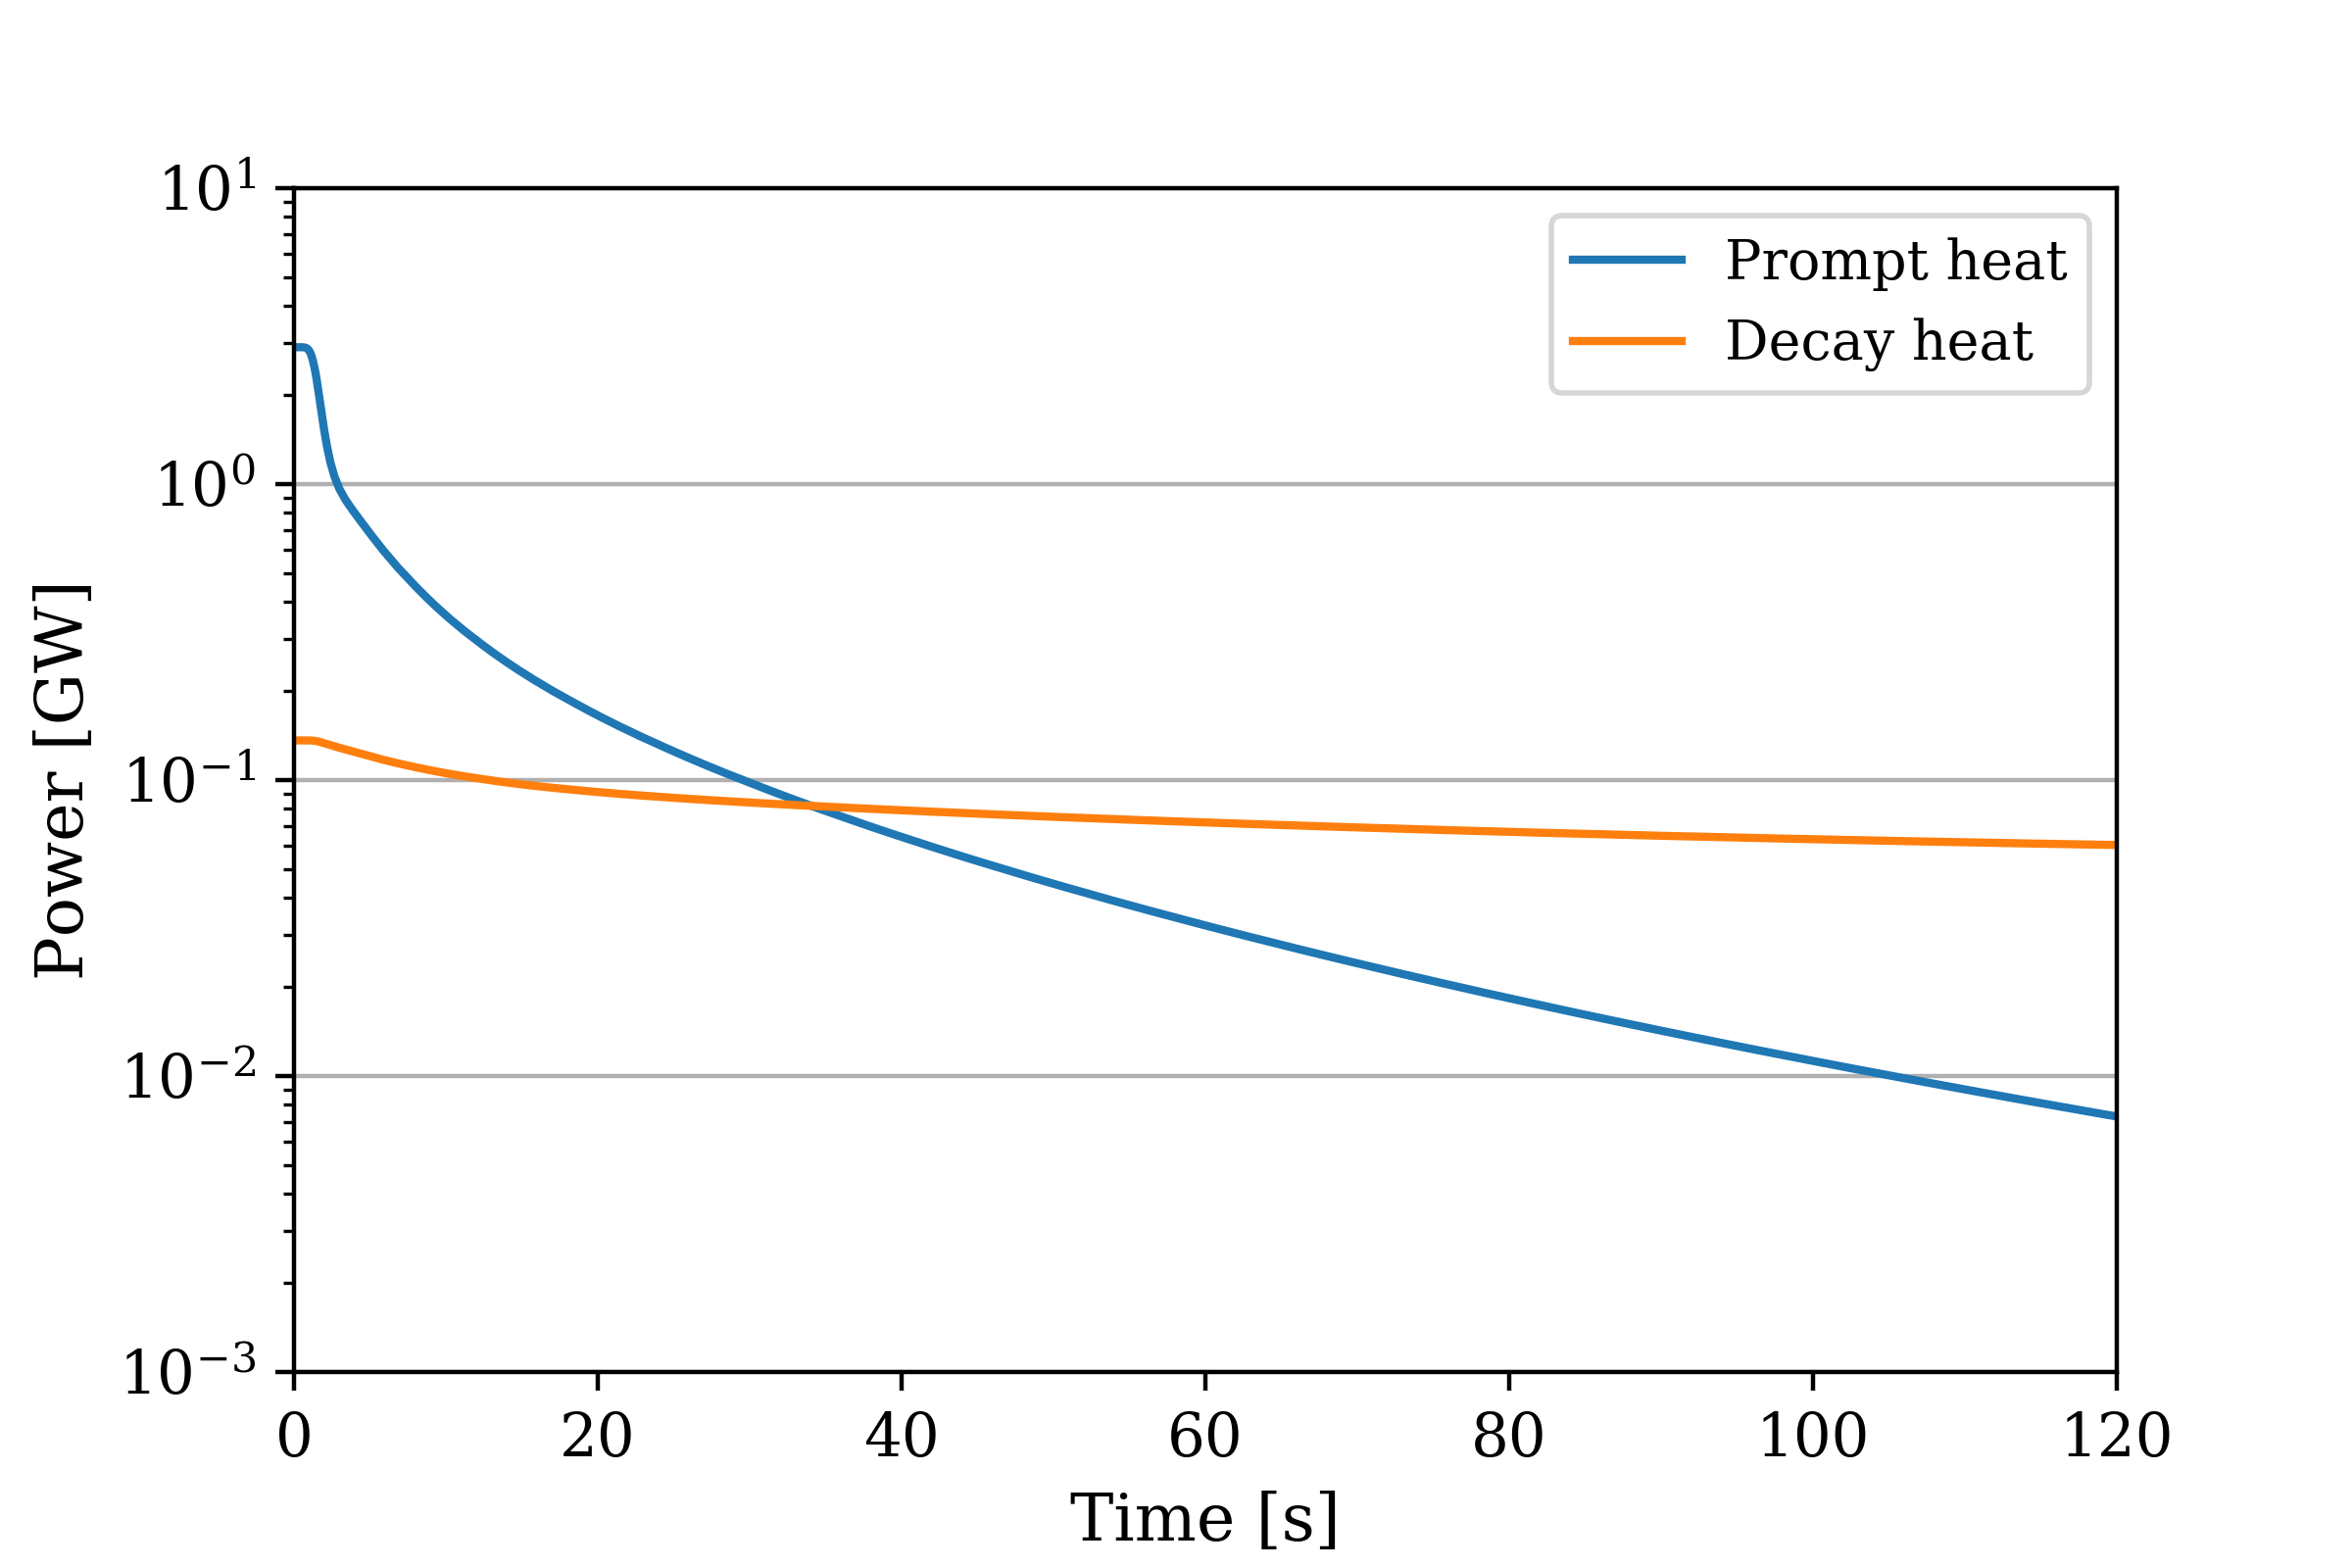
\includegraphics[width=.85\textwidth]{moltres-decay-power}
    \caption{Power output during
    an unprotected loss of heat sink transient in the Moltres model with and
    without decay heat.}
    \label{fig:moltresdecaypower}
    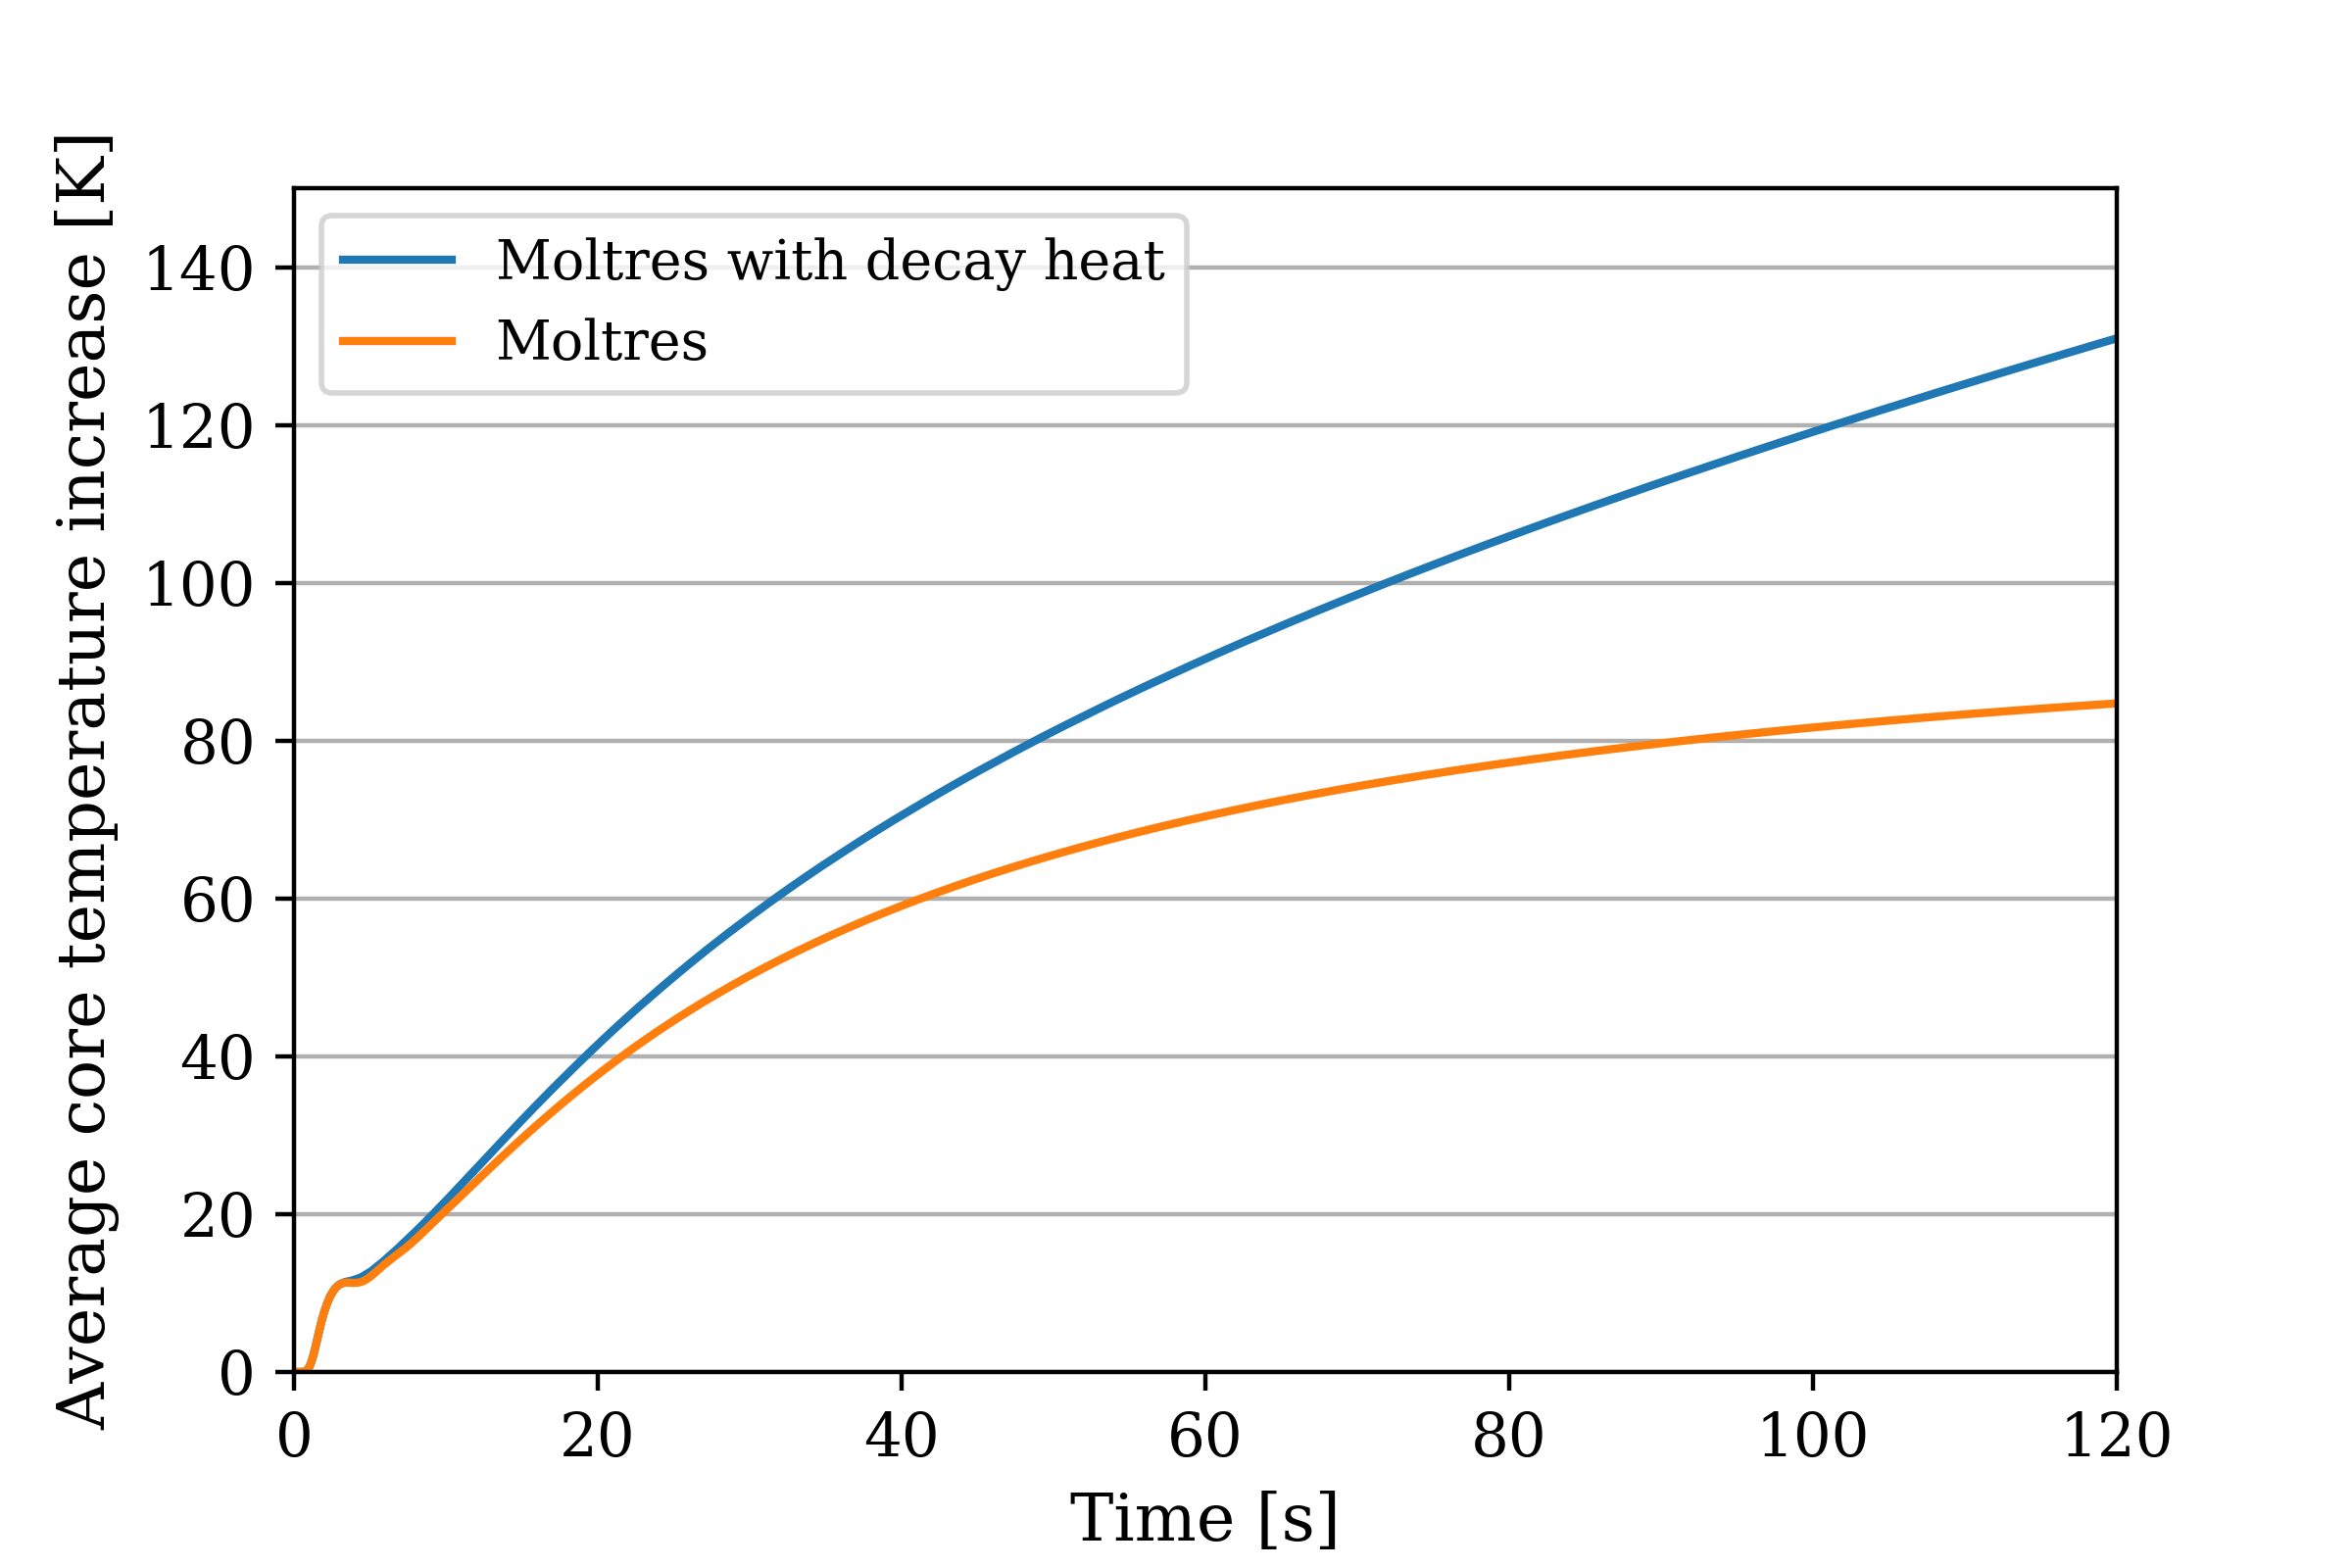
\includegraphics[width=.85\textwidth]{moltres-decay-temp}
    \caption{Average core temperature increase during
    an unprotected loss of heat sink transient in the Moltres model with and
    without decay heat.}
    \label{fig:moltresdecaytemp}
\end{figure}

\clearpage

\begin{figure}[htbp!]
    \centering
    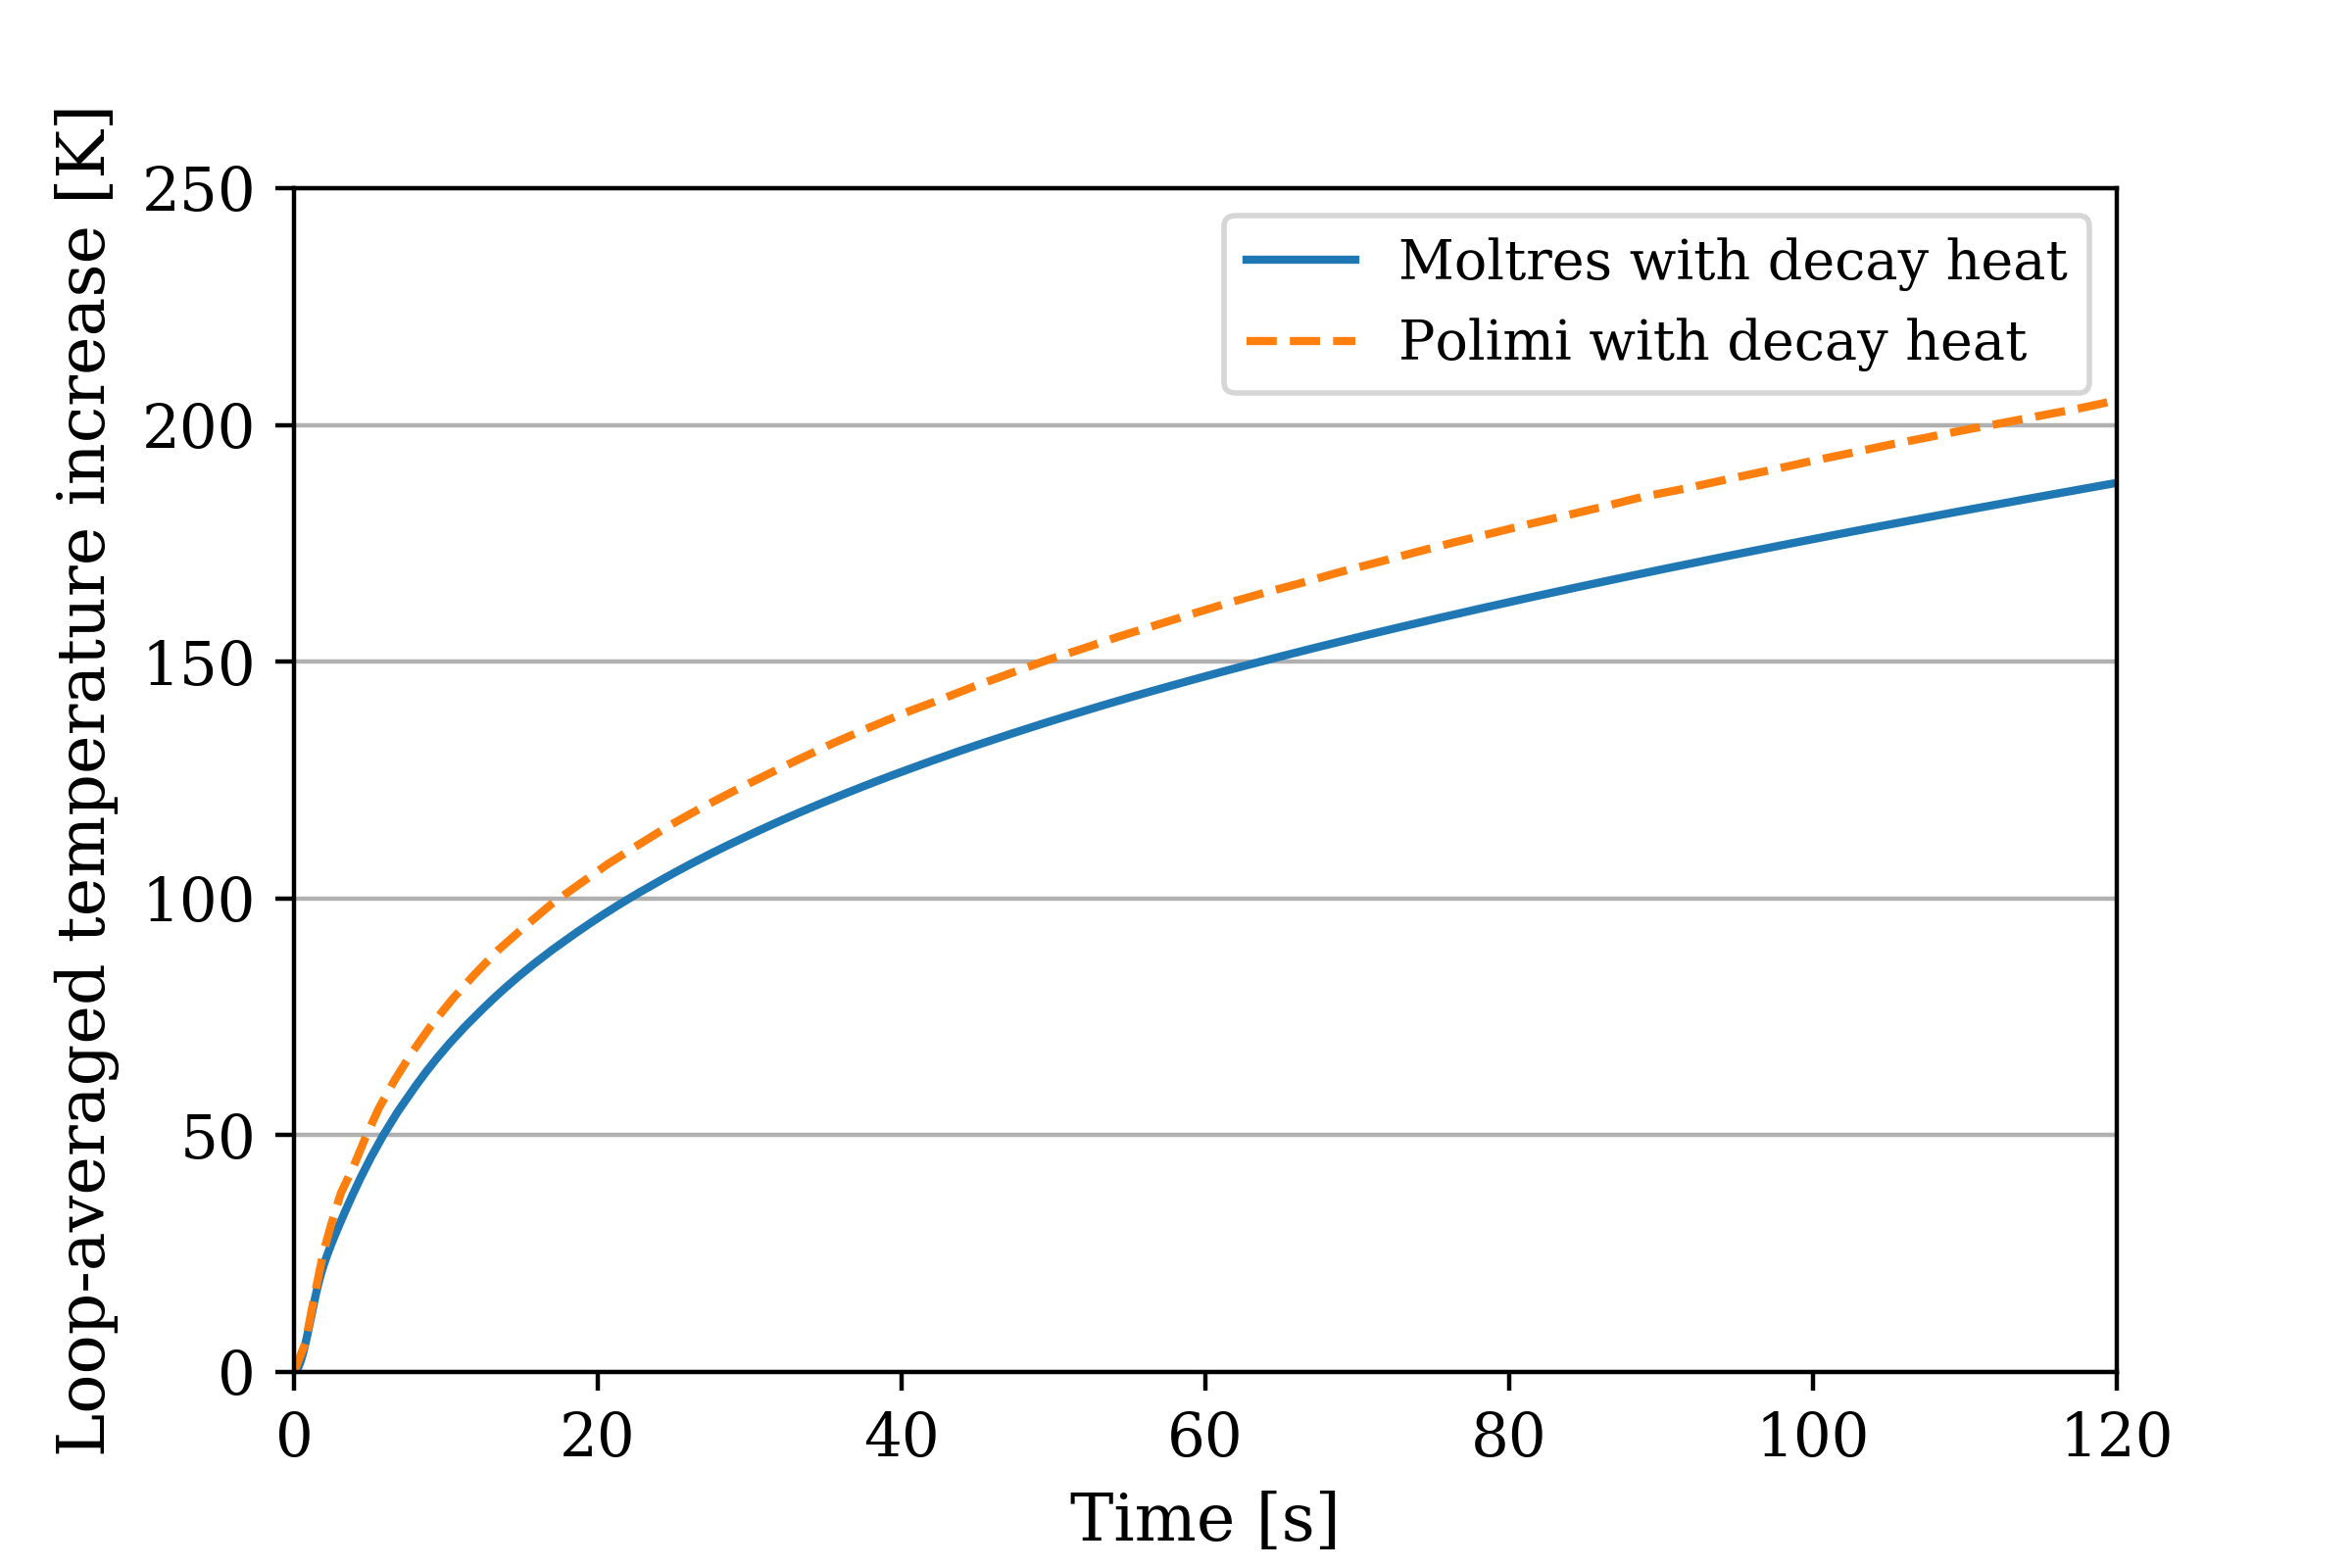
\includegraphics[width=.85\textwidth]{decay-temp}
    \caption{Loop-averaged temperature increase during
    an unprotected loss of heat sink transient in the Moltres and Polimi
    models \cite{fiorina_modelling_2014} with decay heat.}
    \label{fig:polimidecaytemp}
\end{figure}

\section{Unprotected Loss of Flow}

A loss of forced flow transient can occur in the event of a station
blackout; the pumps would cease operating due to the loss of AC electrical
power. Natural circulation resulting from temperature-dependent density
changes becomes the dominant driving force for salt flow in the primary loop.
Fiorina et al. \cite{fiorina_modelling_2014} applied the Boussinesq
approximation for buoyancy-driven flow in their models, but this approach was
not possible in Moltres because the primary loop is partitioned into two
separate geometries and used Dirichlet boundary
conditions at the inlet to drive flow. Fiorina et al.'s Polimi and TUDelft
models featured complete exponential coast-downs of the pumps with a time
constant of 5 s. The resulting flow rate $\dot{m}$ from natural circulation
was approximately 18 times smaller than the initial $\dot{m}$. Figure
\ref{fig:flowrate} shows that the actual $\dot{m}$ decreased with a time
constant of 8 s. Thus, for the \gls{MSFR} model in Moltres, this work imposed
a similar exponential decay term with a time constant of 8 s on the inflow
Dirichlet boundary condition:
%
\begin{align}
    \text{Flow rate, } v = 0.25862 + (4.5-0.25862) e^{-t/8} 
    \label{eq:flowrate}
\end{align}

\begin{figure}[htbp!]
    \centering
    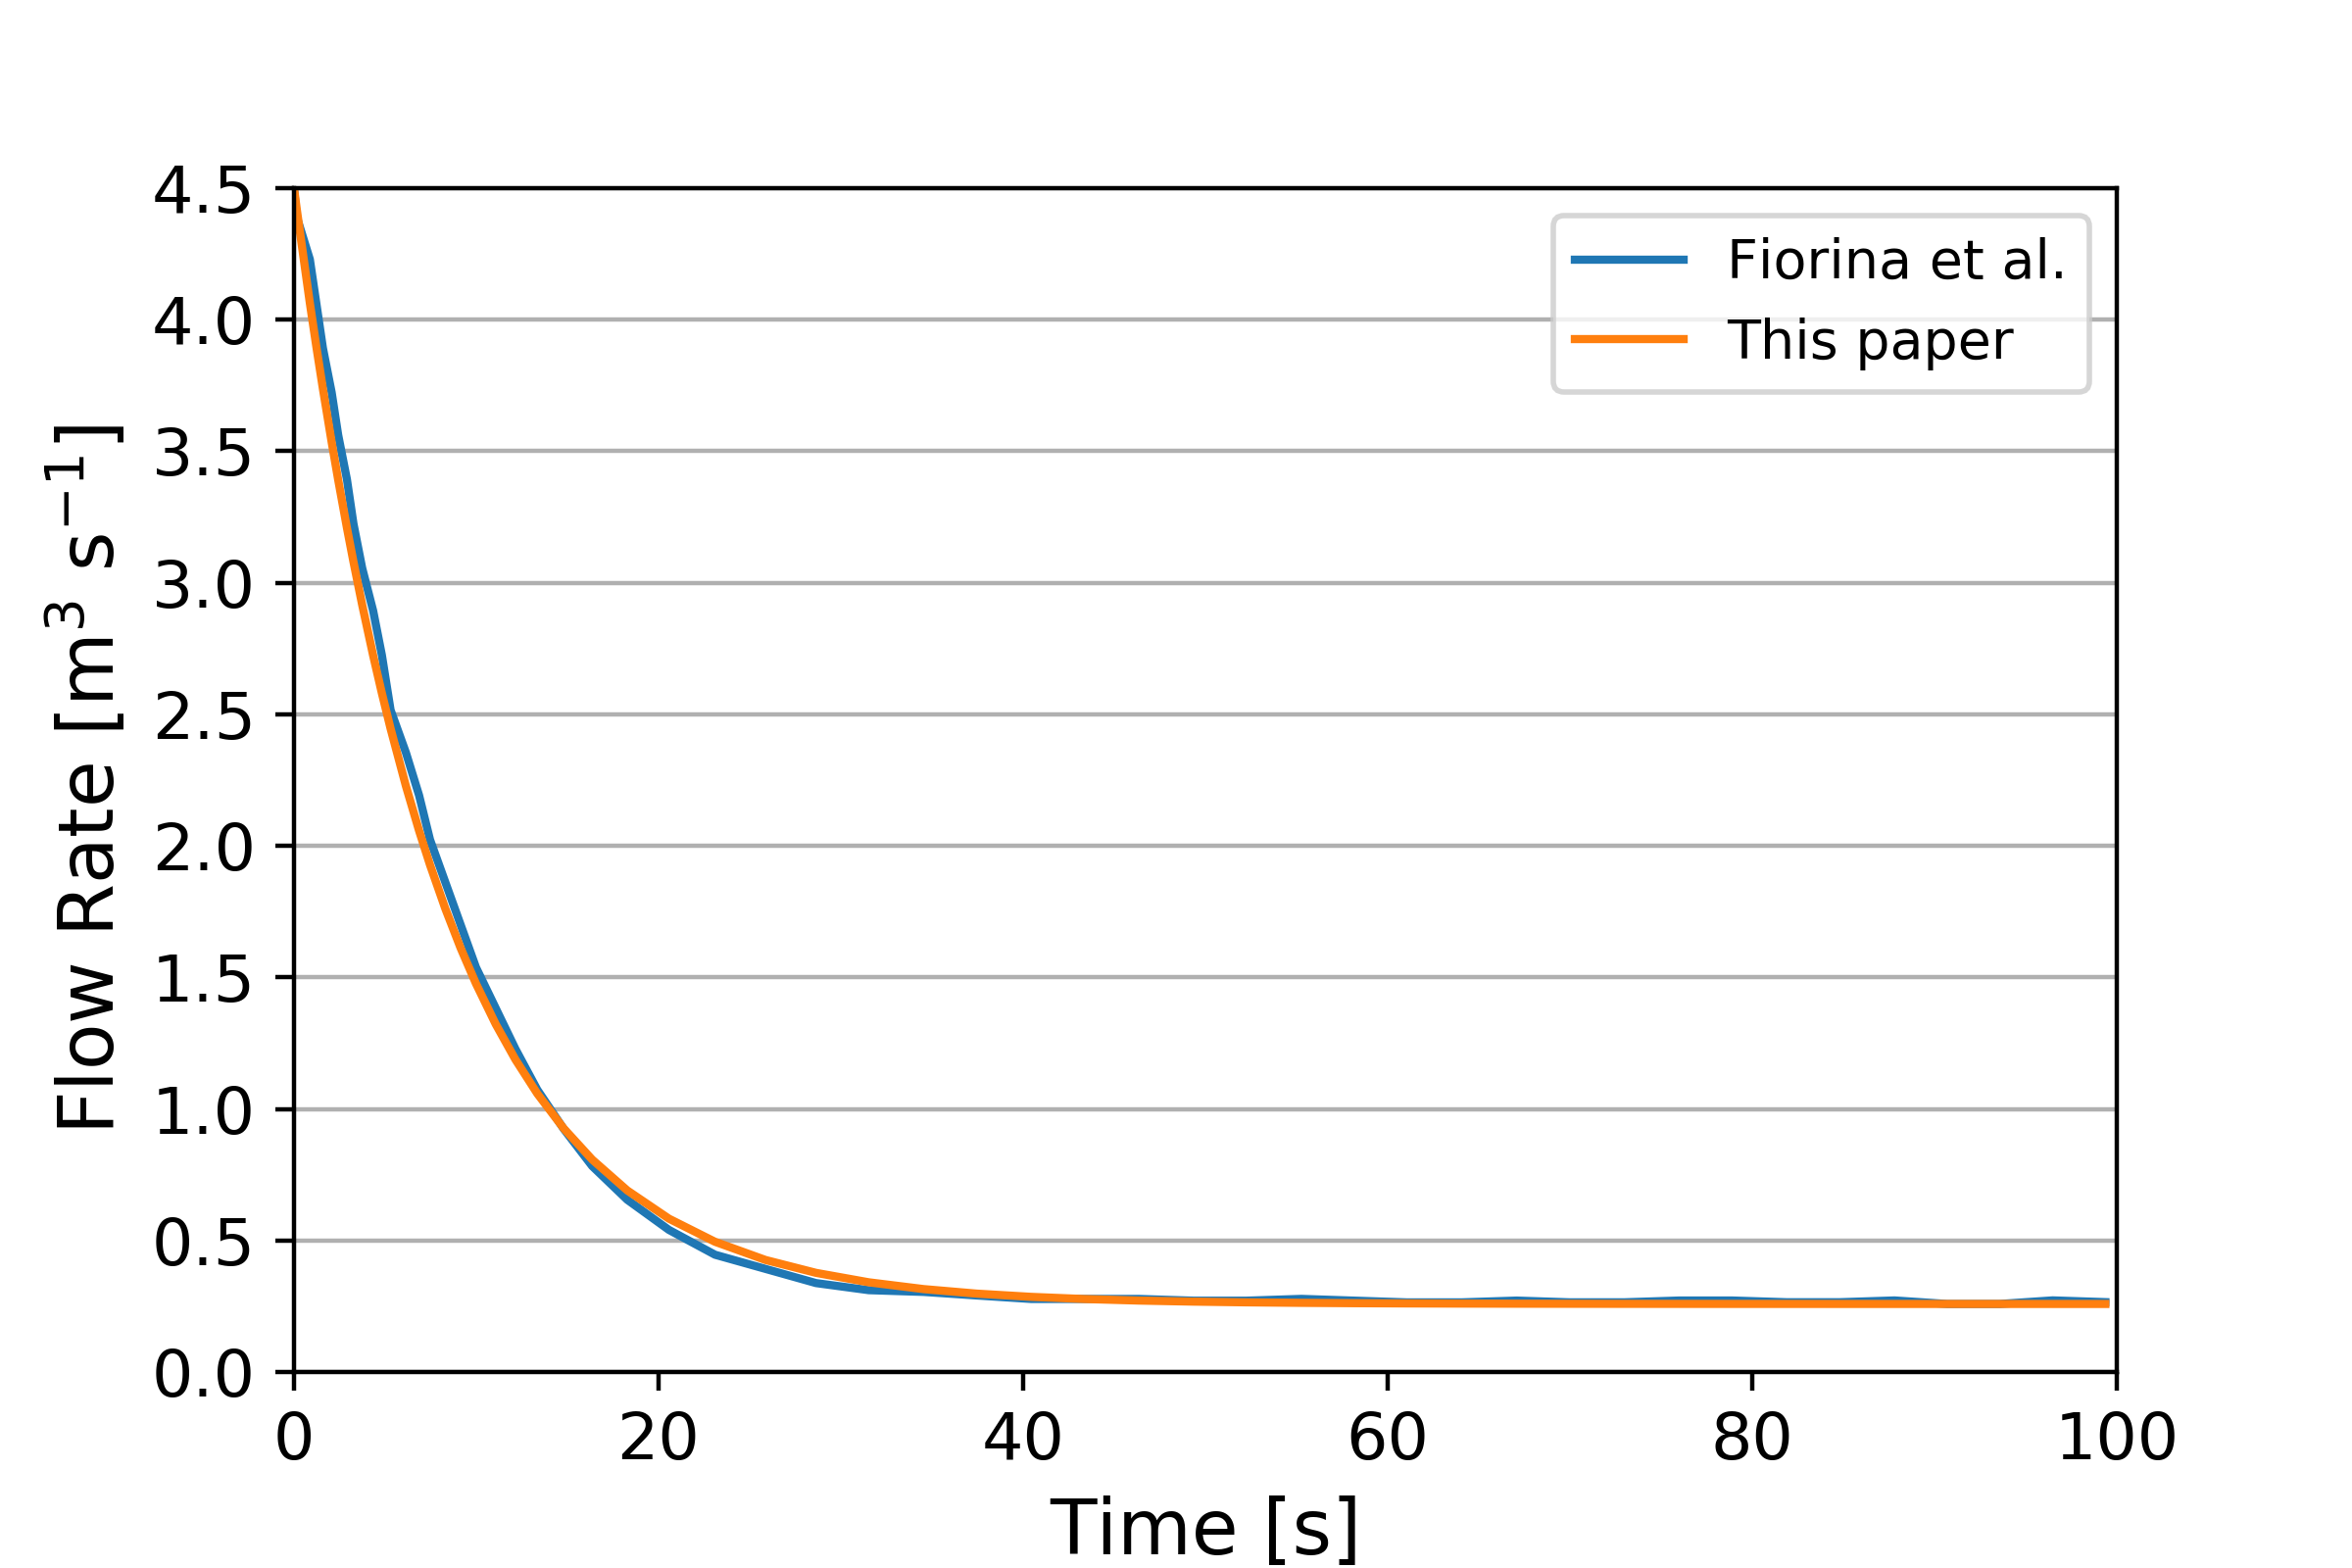
\includegraphics[width=.7\textwidth]{lof-flow-rate}
    \caption{The change in flow rate in the Polimi and TUDelft models and the
    imposed flow rate in Moltres.}
    \label{fig:flowrate}
\end{figure}

The reduced $\dot{m}$ also decreases the heat transfer rate between the
primary and intermediate loop through the heat exchanger as the heat transfer
coefficient $h$ is dependent on the $\dot{m}$. This step was problematic
because
the pointwise heat exchanger implementation in Moltres performs differently
compared with the heat exchangers that take up ``36\% of the out-of-core
part'' in the Polimi and TUDelft models \cite{fiorina_modelling_2014}. Most of
the cooling happens in the top half of the heat exchanger where the
temperature differential between the primary and intermediate loops is the
largest. In the Polimi and TUDelft models, the overall $h$ is the
``harmonic mean of the heat transfer coefficients on each side of the heat
exchanger''. For this loss of flow transient, the authors intended to focus on
the primary loop and assumed that only the pumps in the primary loop failed.
In addition to this, the authors applied the Dittus-Boelter correlation
\cite{dittus_heat_1930} for the relationship between the primary side $h$ and
$\dot{m}$. The Dittus-Boelter correlation for fluids being cooled is:
%
\begin{align}
    Nu &= 0.023 Re^{0.8} Pr^{0.3} \label{eq:db} \\
    \intertext{where}
    Nu &= \text{ Nusselt number,} \nonumber \\
    Re &= \text{ Reynolds number,} \nonumber \\
    Pr &= \text{ Prandtl number.} \nonumber
\end{align}
%
The only direct relation to $\dot{m}$ in the Dittus-Boelter correlation is
through the $Re$ term, which is directly proportional to flow velocity $v$.
This gives the following relation between $h$ and$v$:
%
\begin{align}
    h \propto v^{0.8} \label{eq:hv}
\end{align}
%
However, this relation provided very different results in the unprotected loss
of flow and pump overspeed transients compared with the Polimi and TUDelft
models; it overpredicted the equilibrium power output in the
unprotected loss of flow transient and underpredicted the same parameter in
the unprotected pump overspeed transient. Upon further investigation, the
present author found that raising the power of $v$ from 0.8 to 1.1 brought the
average core temperatures closer to the results from the other models in both
transients. Therefore, this work adopted the raised power in this study.

Another issue pertained to the turbulent viscosity $\mu_t$ as a function of
$v$. Using a simple approximation of $\mu_t$ being directly
proportional to $v$, the results differed significantly compared with the
Polimi and TUDelft models. This is likely due to buoyancy-driven flow
contributing to turbulence; the turbulent energy $k$ equation in COMSOL's
$k$-$\epsilon$ model has an explicit source term from buoyancy effects
\cite{comsol_ab_comsol_2018}. Another point to note is the
Reynolds number remains constant if $\mu$ and $v$ decrease in tandem. This
preserves the existence of the recirculation zone in the core and it is at
odds with the results from the Polimi and TUDelft models, which show that the
recirculation zones disappear during the loss of flow transient. We
circumvented this issue by letting fixed fractions of the initial $\mu_{t,0}$
be conserved regardless of the final flow velocity, according to the following
equation:
%
\begin{align}
    \mu_t &= \mu_c + (\mu_{t,0} - \mu_c) e^{-t/8} \label{lofmu} \\
    \intertext{where}
    \mu_c &= \text{ conserved fraction of $\mu_{t,0}$ [Pa$\cdot$s].} \nonumber
\end{align}
%
This measure allowed for laminar flow to develop in the core and yielded
results with closer resemblance to those from the Polimi and TUDelft models.

Figures \ref{fig:lofheat} and \ref{fig:loftemp} show the power output and
average core temperature increase during the unprotected loss of flow
transient in the Moltres, Polimi, and TUDelft models without decay heat
modeling. The three sets of results from Moltres correspond to $\mu_c =
\frac{1}{4} \mu_{t,0}, \frac{1}{2} \mu_{t,0}, \text{and } \frac{3}{4}
\mu_{t,0}$. Moltres
performs poorer in this transient relative to the two previous transients.
Although Moltres shows the same decreasing trend in power output, it failed to
capture the exact individual features in the reactor response. In the Polimi 
and TUDelft models, Fiorina et al.
stated that after around $t=15$ s, the ``flow pattern changed in the core and
the recirculation zones started to disappear''. A sudden drop in the average
core temperature results as the pocket of hot salt leaves the
core. In Moltres, the wider peak in the average core temperature
indicates that there was a more gradual change in the flow pattern.

Figure \ref{fig:lofflowtemp} shows the flow patterns and temperature
distribution in the core at $t=300$ s in all three models. Figures
\ref{fig:lofheat}, \ref{fig:loftemp}, and \ref{fig:lofflowtemp} combined
highlight the difference between laminar flow in the Moltres model and
buoyancy-driven flow in the other models, and its impact on the reactor
response. They show that low-speed laminar flow is a poor substitute for
buoyancy-driven flow in the context of the MSFR. It is particularly evident
in the transition from high-speed turbulent flow to low-speed viscous
flow as Moltres mispredicted the intermediate stages. The
simplifying assumption for the uniform, time-dependent $\mu_t$ is also flawed
in a safety analysis code.

The results from this transient inform our goals for Moltres: 1)
implementing a proper turbulence model, and
2) developing a new heat exchanger feature that is compatible with the
buoyancy-driven flow capabilities already present in Moltres.

\begin{figure}[htbp!]
    \centering
    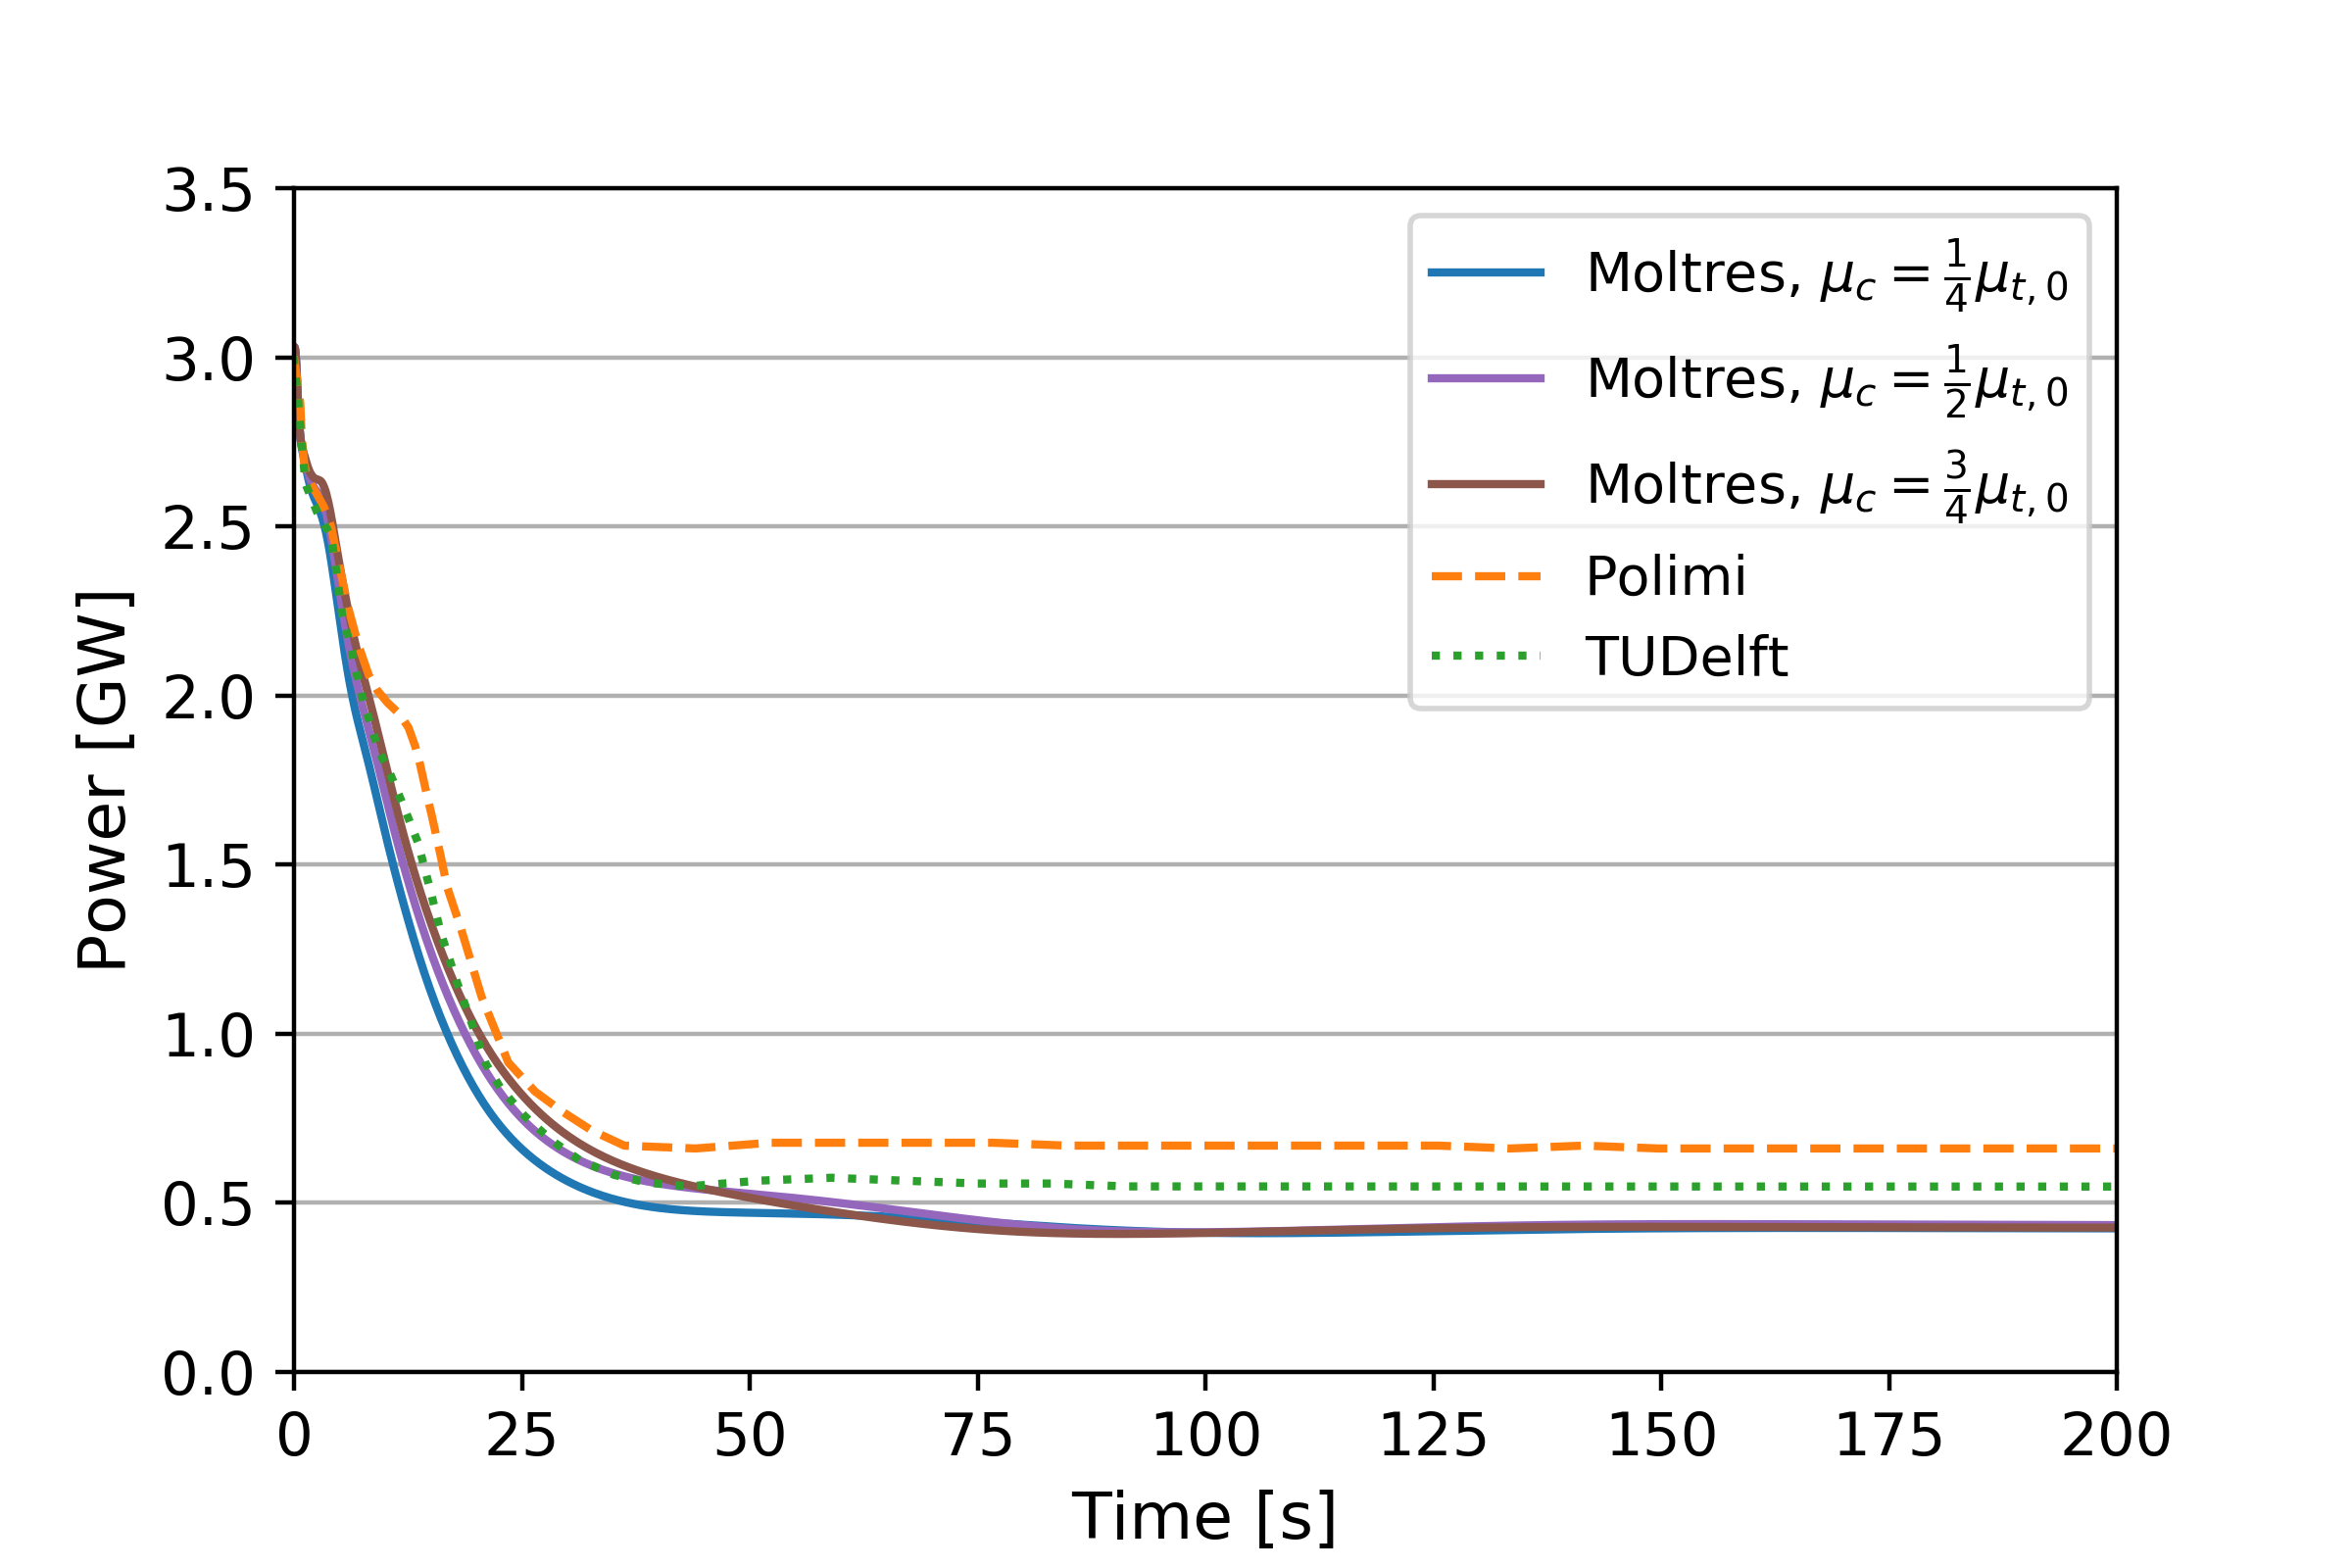
\includegraphics[width=.85\textwidth]{lof-heat}
    \caption{Power output during
    an unprotected loss of flow transient in the Moltres, Polimi, and
    TUDelft models \cite{fiorina_modelling_2014}.}
    \label{fig:lofheat}
    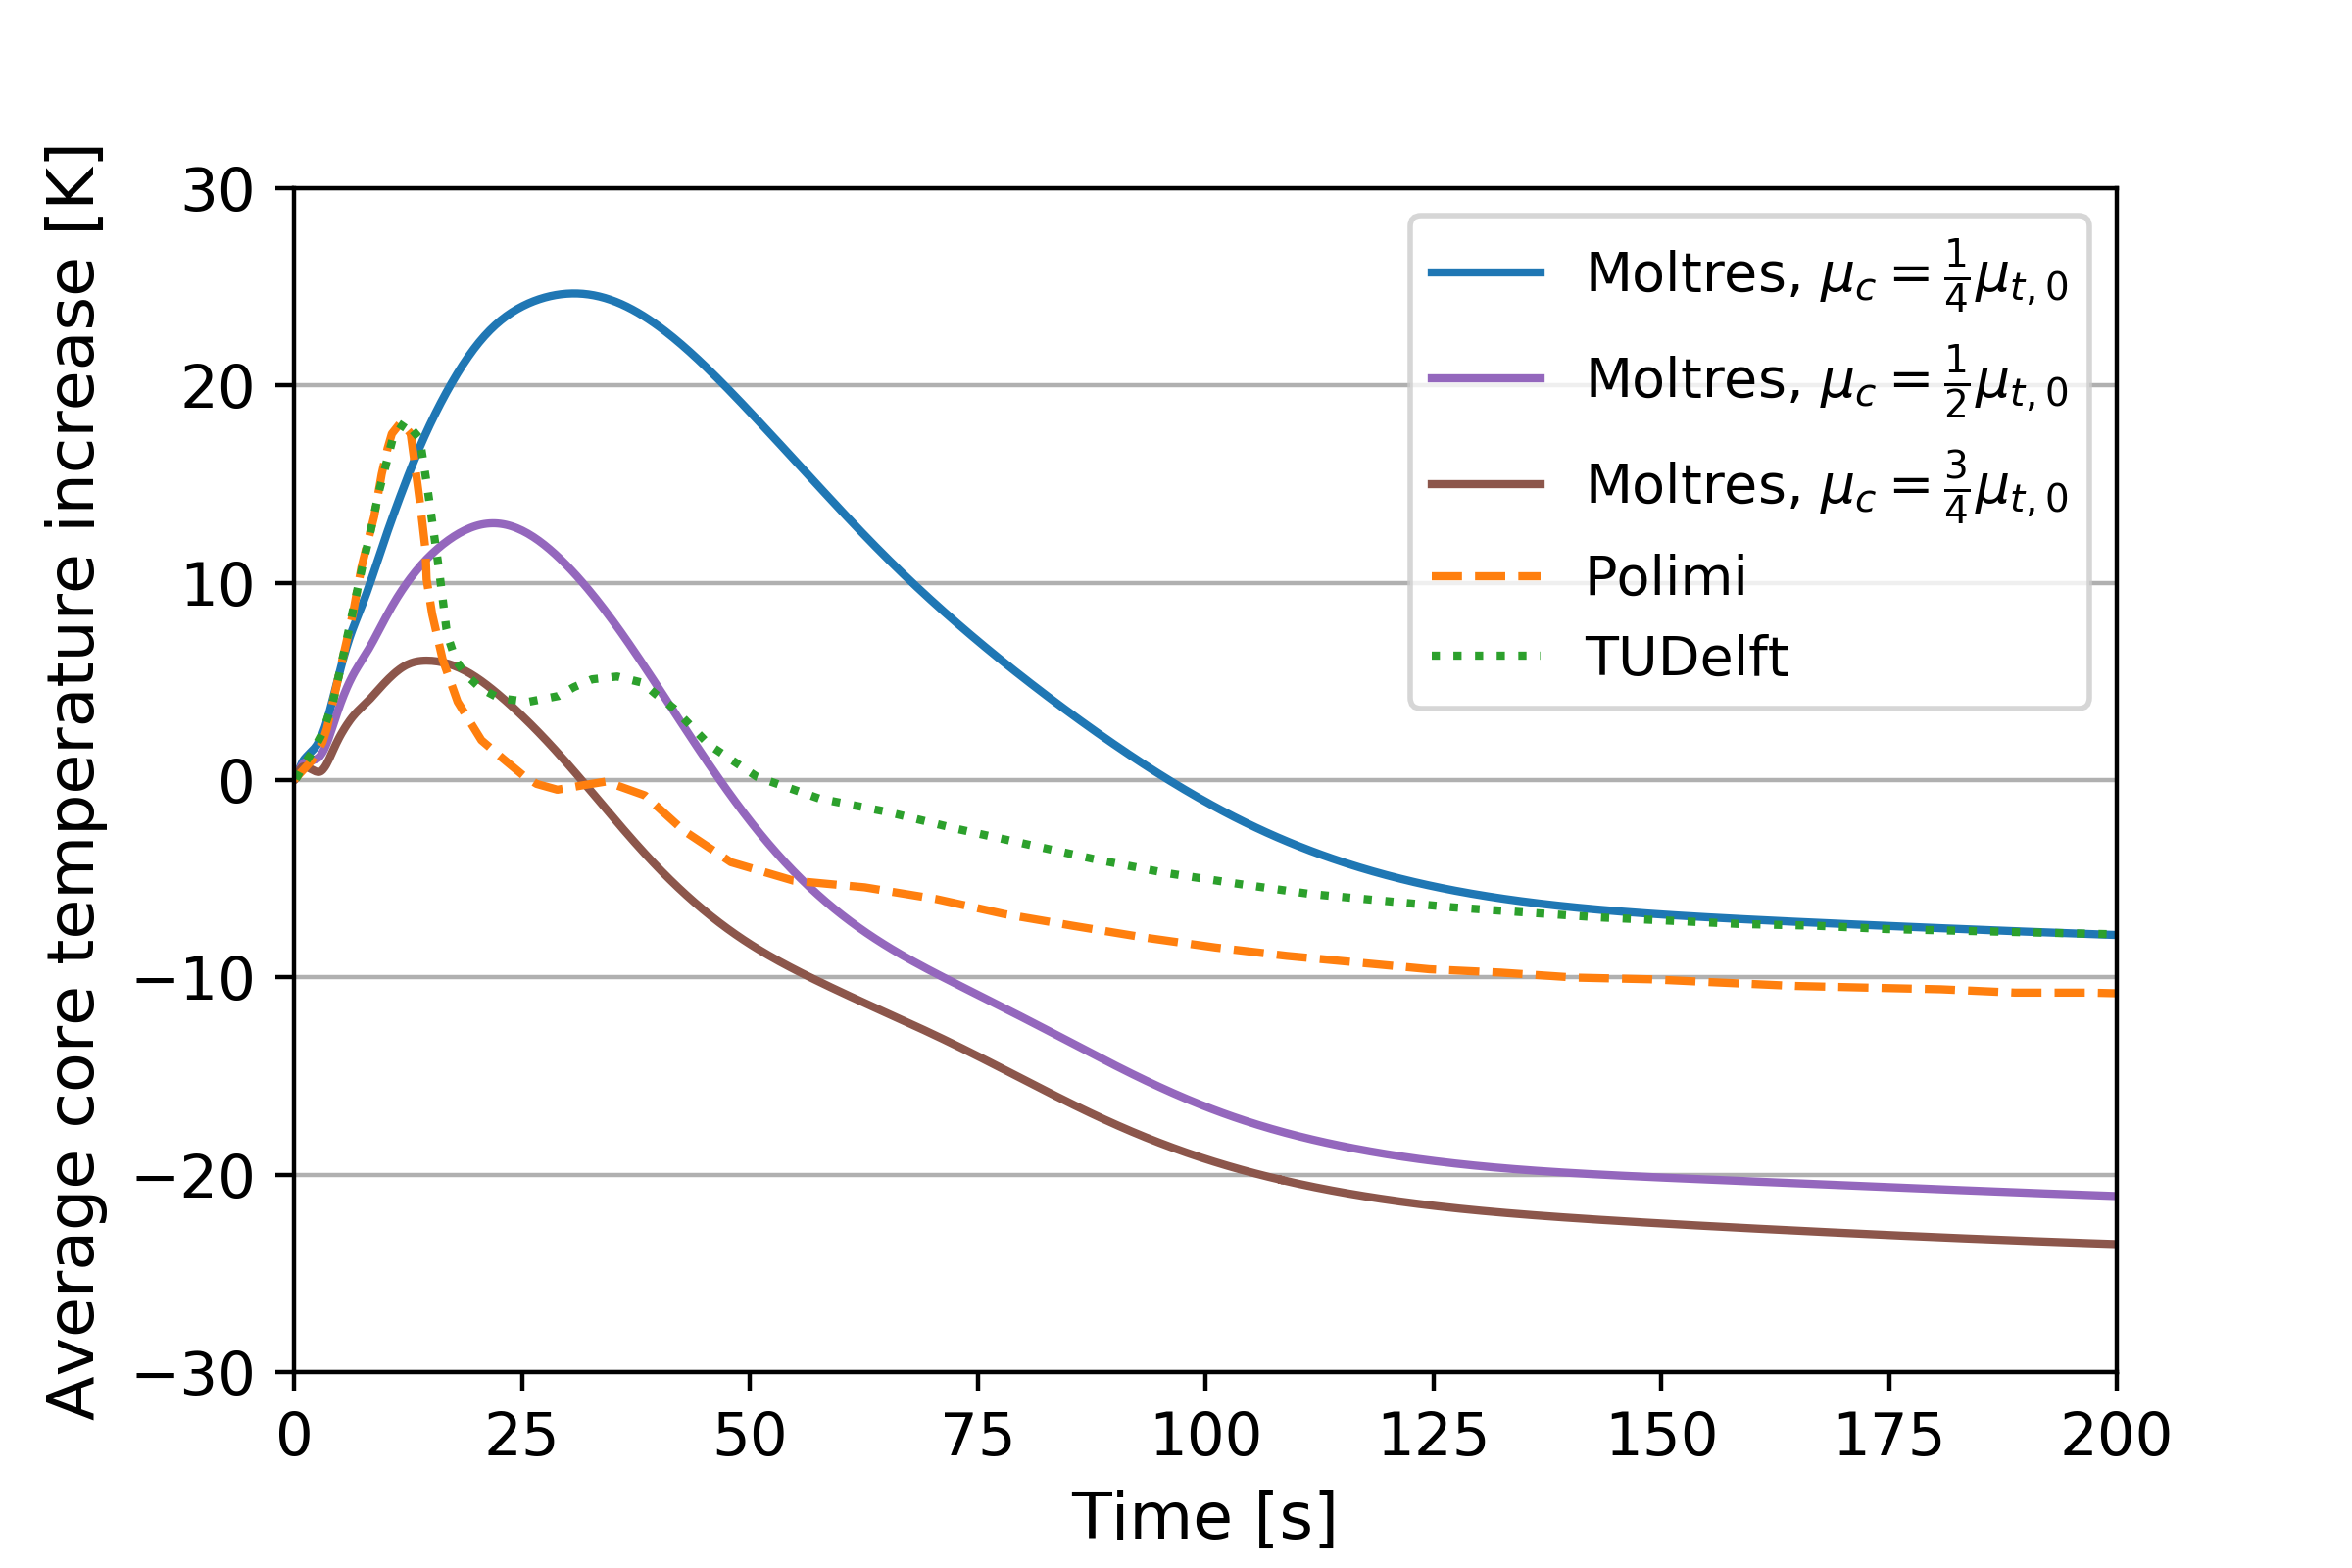
\includegraphics[width=.85\textwidth]{lof-temp}
    \caption{Average core temperature increase during
    an unprotected loss of flow transient in the Moltres, Polimi, and
    TUDelft models \cite{fiorina_modelling_2014}.}
    \label{fig:loftemp}
\end{figure}

\clearpage

\begin{figure}[htbp!]
    \centering
    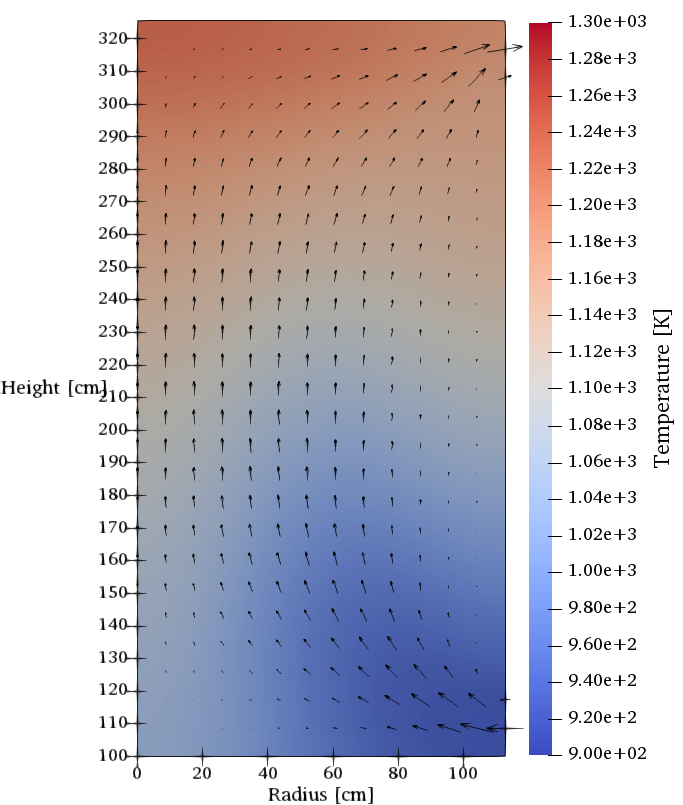
\includegraphics[width=.37\textwidth]{lof-flow-temp}
    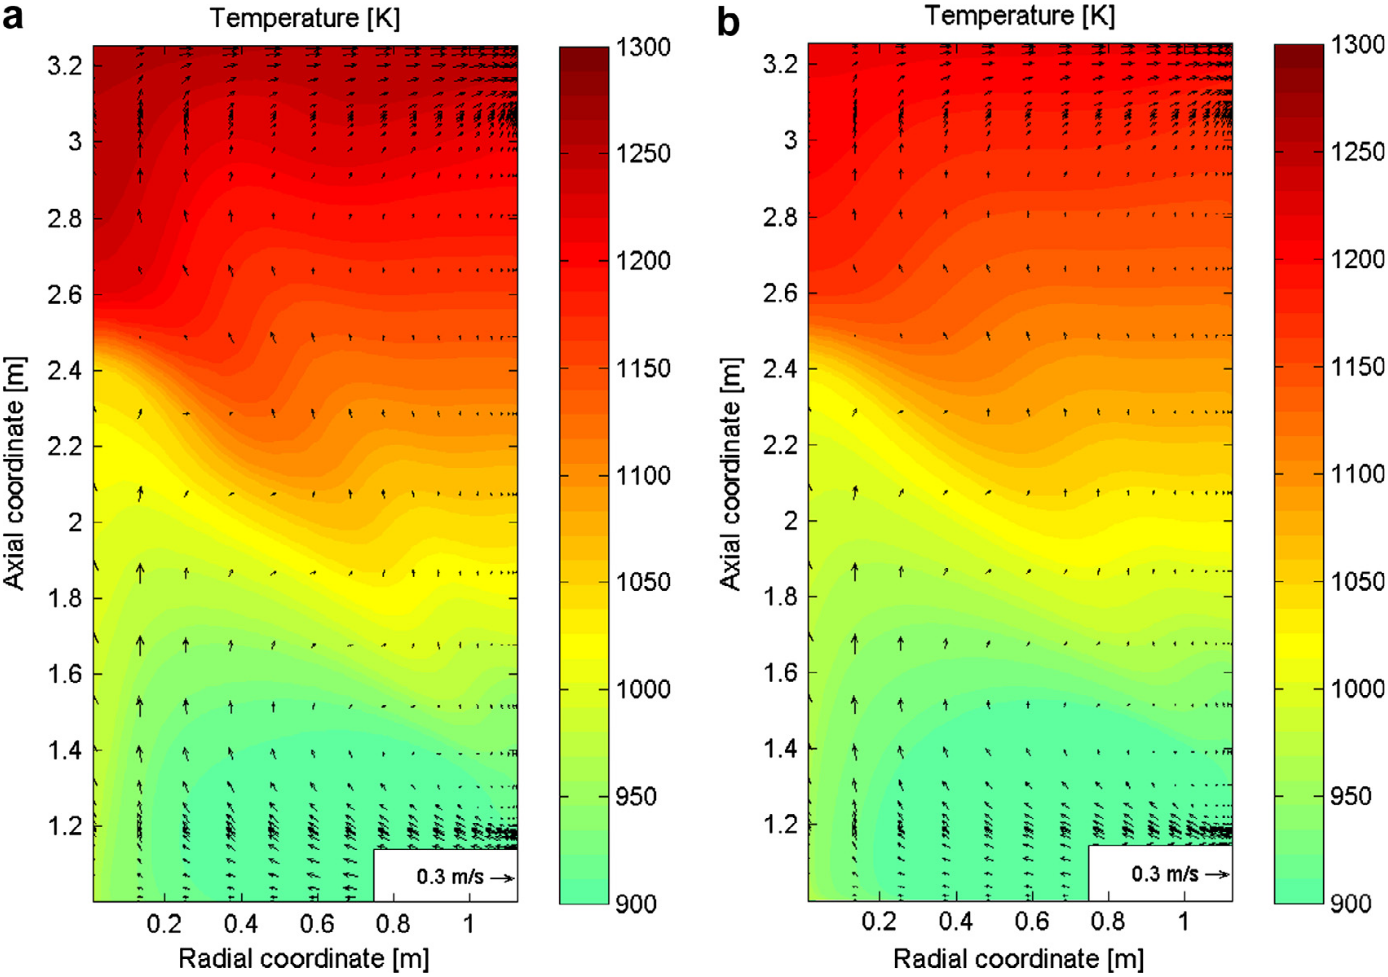
\includegraphics[width=.62\textwidth]{fiorina-lof}
    \caption{Temperature and velocity fields in the core at $t=300$ s during
    a loss of flow transient in the Moltres ($\mu_c = \frac{1}{2} \mu_{t,0}$),
    Polimi, and TUDelft models.}
    \label{fig:lofflowtemp}
\end{figure}

\section{Unprotected Pump Overspeed}

Pump overspeed refers to a sustained
increase in pump speed in the primary coolant loop. The increased flow rate
$\dot{m}$ impacts reactor performance in several ways.
It affects the neutronics by reducing the in-core $\beta$ as more of the
shorter-lived precursors will tend to flow out of the core before decaying.
This net loss of neutrons reduces the reactivity in the core, thereby causing
core temperatures to fall to counteract this change through temperature
reactivity feedback. The increased $\dot{m}$ also enhances the heat transfer
coefficient on the primary loop side of the heat exchanger and enables the
reactor to operate at a higher power output. At the same time, the improved
mixing flattens the temperature distribution in the core.

This workfollowed Fiorina et al.'s implementation
\cite{fiorina_modelling_2014} by
ramping up the inlet velocity, $u$, by 50\% from the nominal value, $u_0$,
according to the following formula:
%
\begin{align}
    u(t) &= u_0 [1 + 0.5 (1 - e^{-t / \tau})] \label{eq:overspeed}
    \intertext{where}
    \tau &= 5 \text{ s.} \nonumber
\end{align}
%
For this transient, this work assumed that $\mu_t$ was directly proportional
to $v$ because the buoyancy effects are negligible and the recirculation zones 
persist throughout the entire duration. Figures \ref{fig:poheat} and
\ref{fig:potemp} show the power output and average core temperature increase
during the unprotected pump overspeed transient in the Moltres, Polimi, and
TUDelft models. Figure \ref{fig:poshort} shows the same results for the first
20 seconds of the transient. At the start of the transient, the rising flow
rate cools the core and causes power output to rise sharply. Although the
average core temperature has a strictly decreasing trend, the temperature at
the center of the core briefly rises due ot the sharp increase in power
output. Since this is the region where most of the fissions take place, the
Doppler effect and salt expansion causes the power output to stall and dip
briefly before rising again at $t=2.5$ s. The reactor tends to a new
equilibrium power output and average core temperature. The temperature
distribution in the core is more evenly distributed because the turbulent
thermal conductivity $k_t$ is directly proportional to $mu_t$.

\begin{figure}[htbp!]
    \centering
    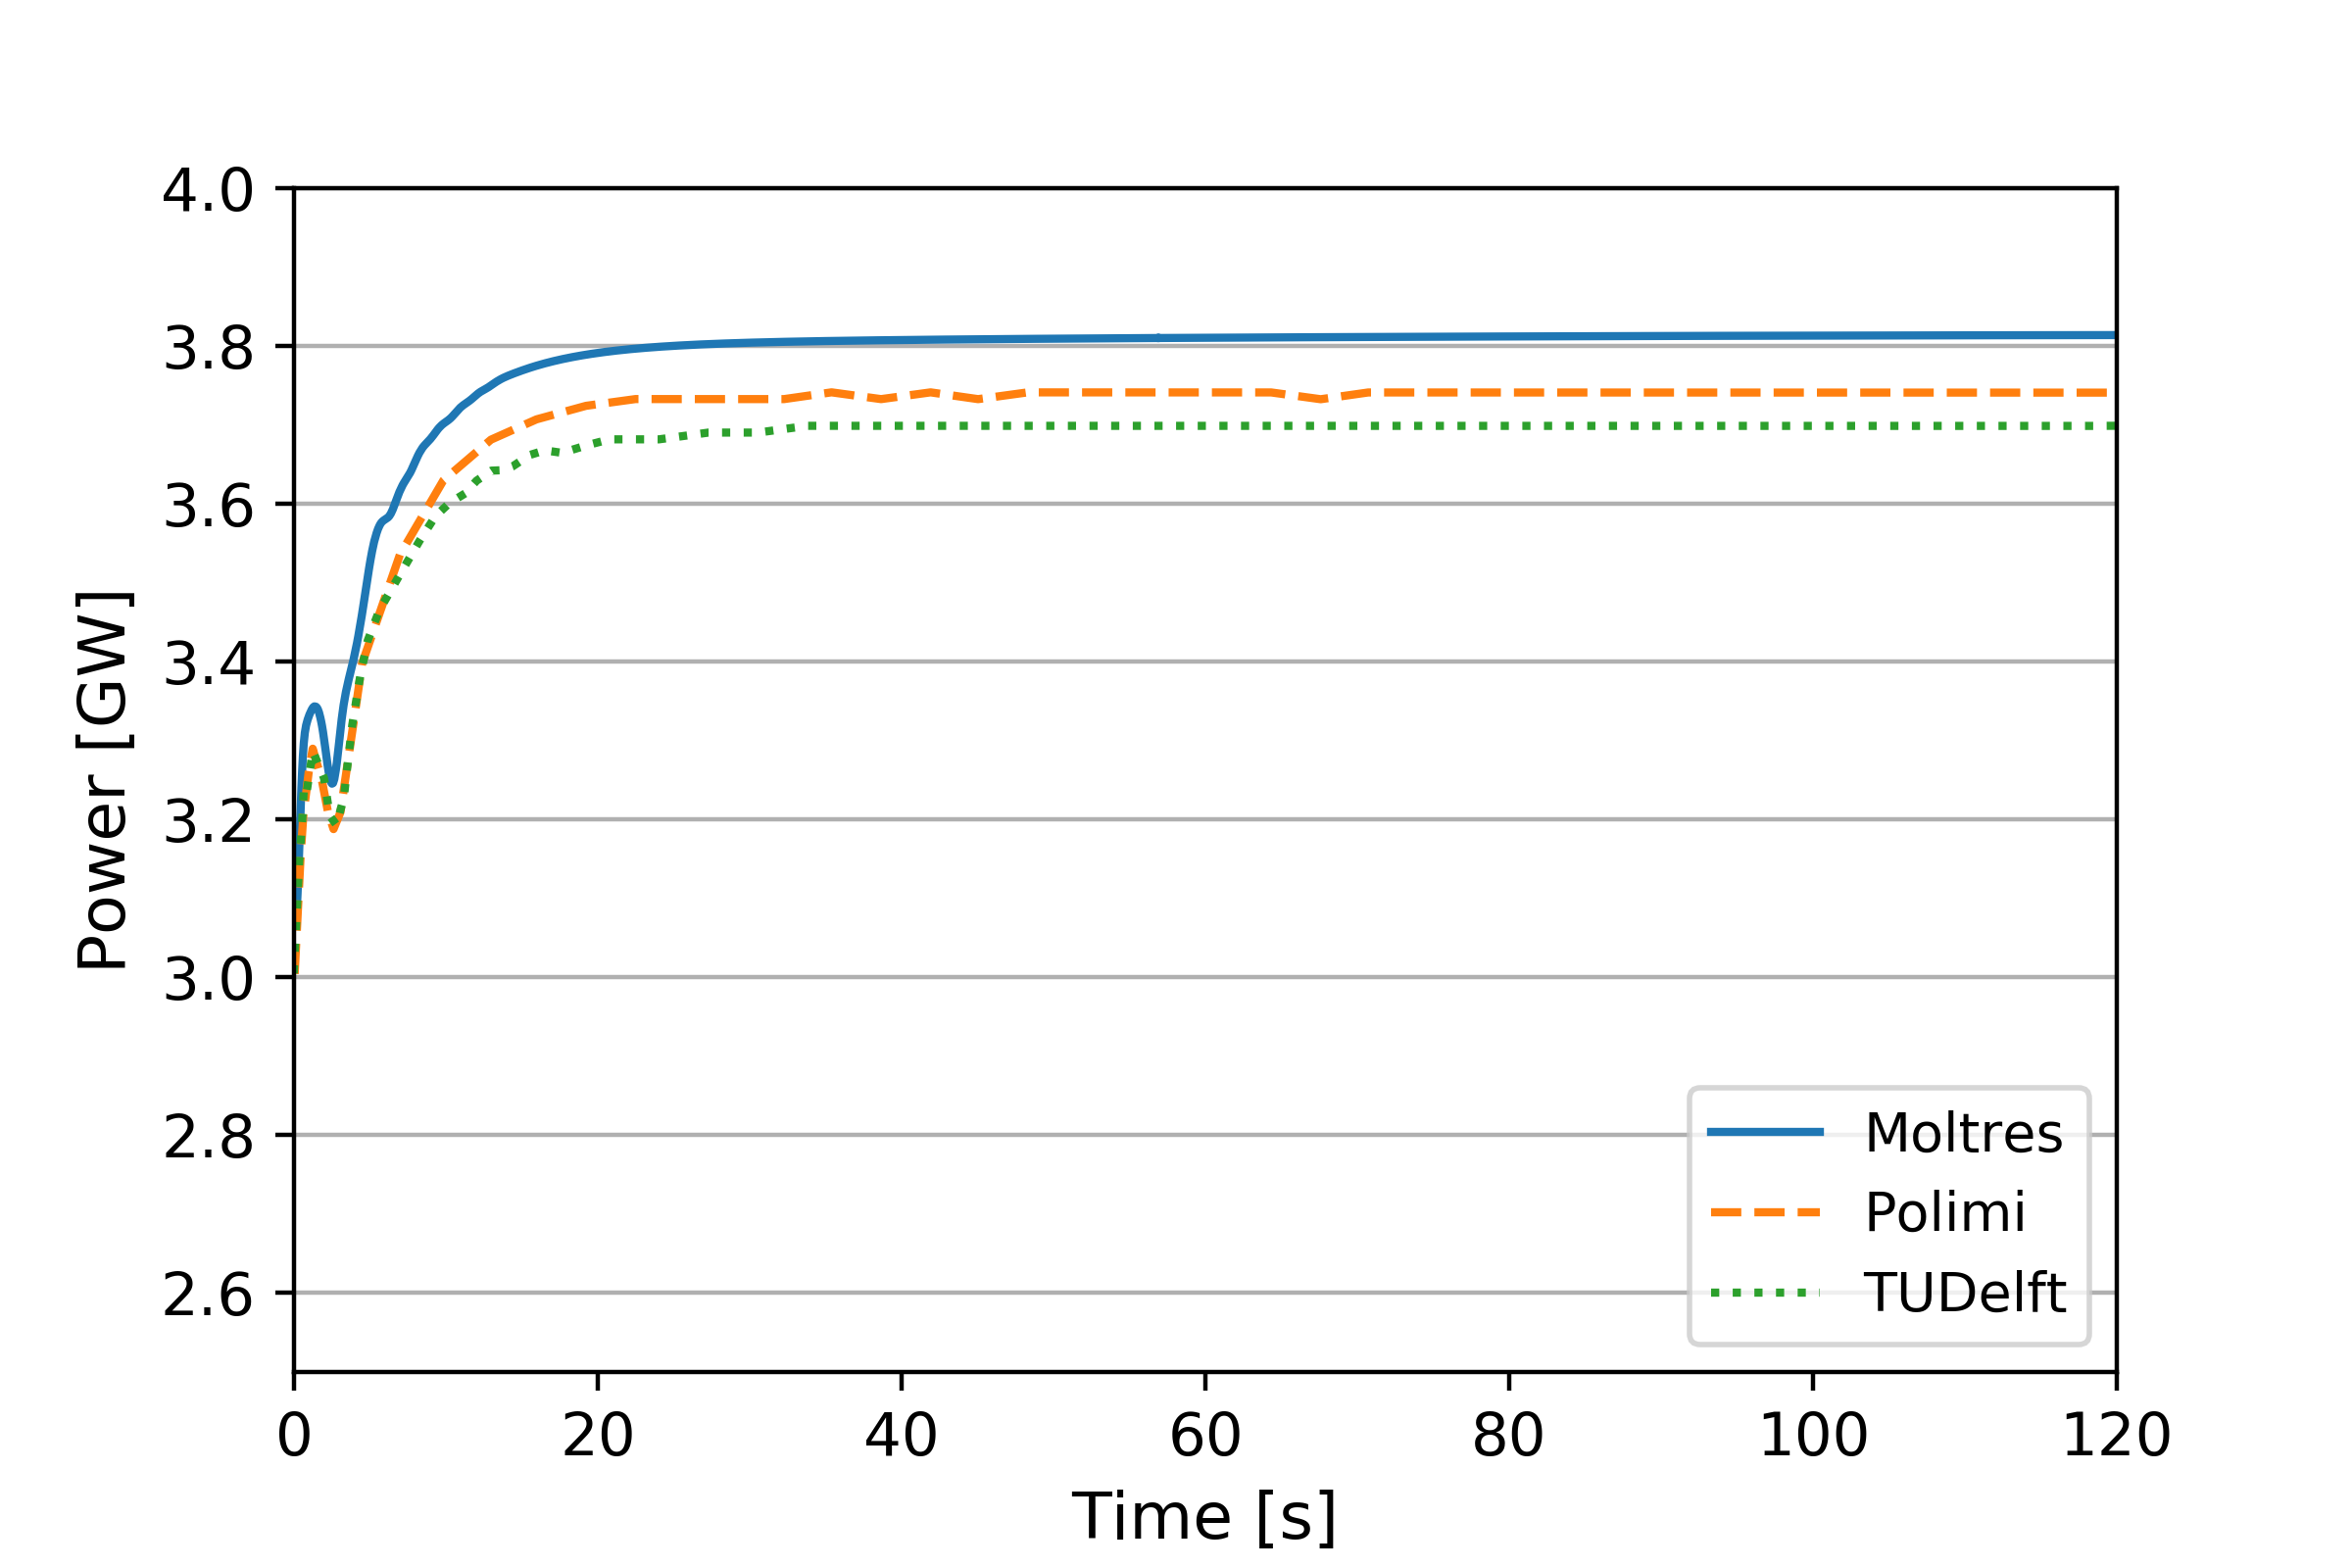
\includegraphics[width=.85\textwidth]{po-heat}
    \caption{Power output during
    an unprotected pump overspeed transient in the Moltres, Polimi, and
    TUDelft models \cite{fiorina_modelling_2014}.}
    \label{fig:poheat}
    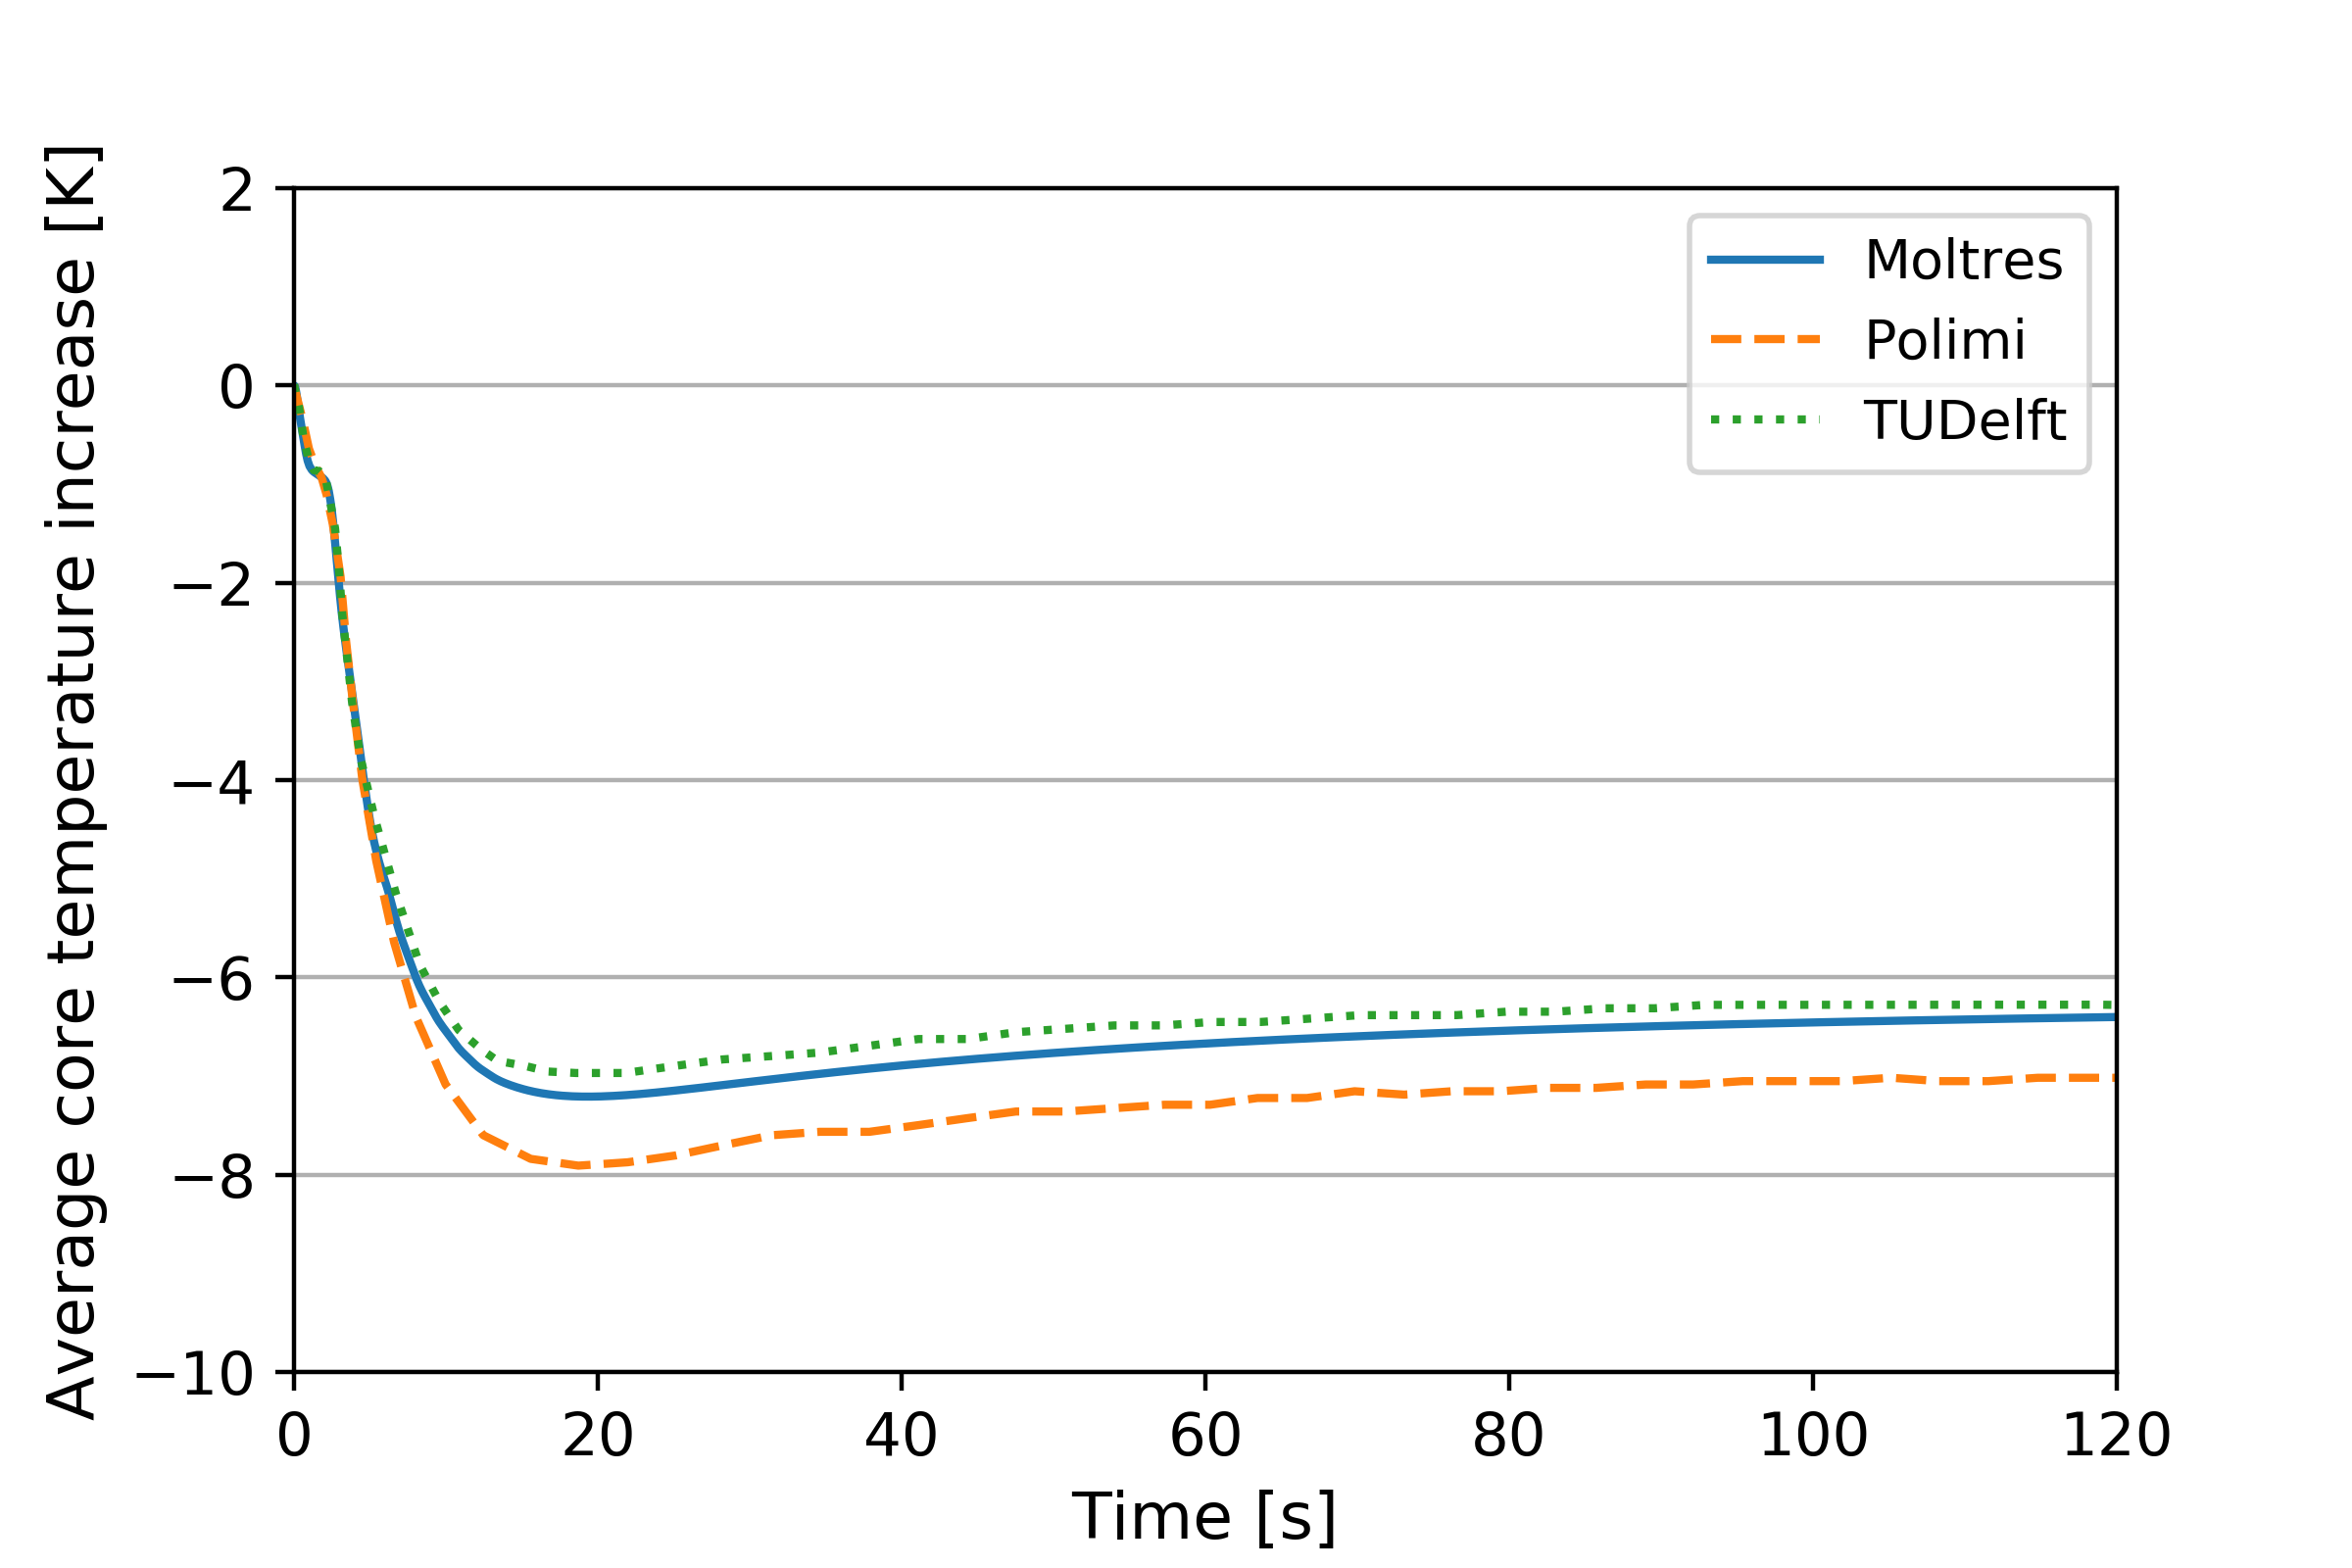
\includegraphics[width=.85\textwidth]{po-temp}
    \caption{Average core temperature increase during
    an unprotected pump overspeed transient in the Moltres, Polimi, and
    TUDelft models \cite{fiorina_modelling_2014}.}
    \label{fig:potemp}
\end{figure}

\begin{figure}[htbp!]
    \centering
    \begin{subfigure}[t]{.485\textwidth}
        \centering
        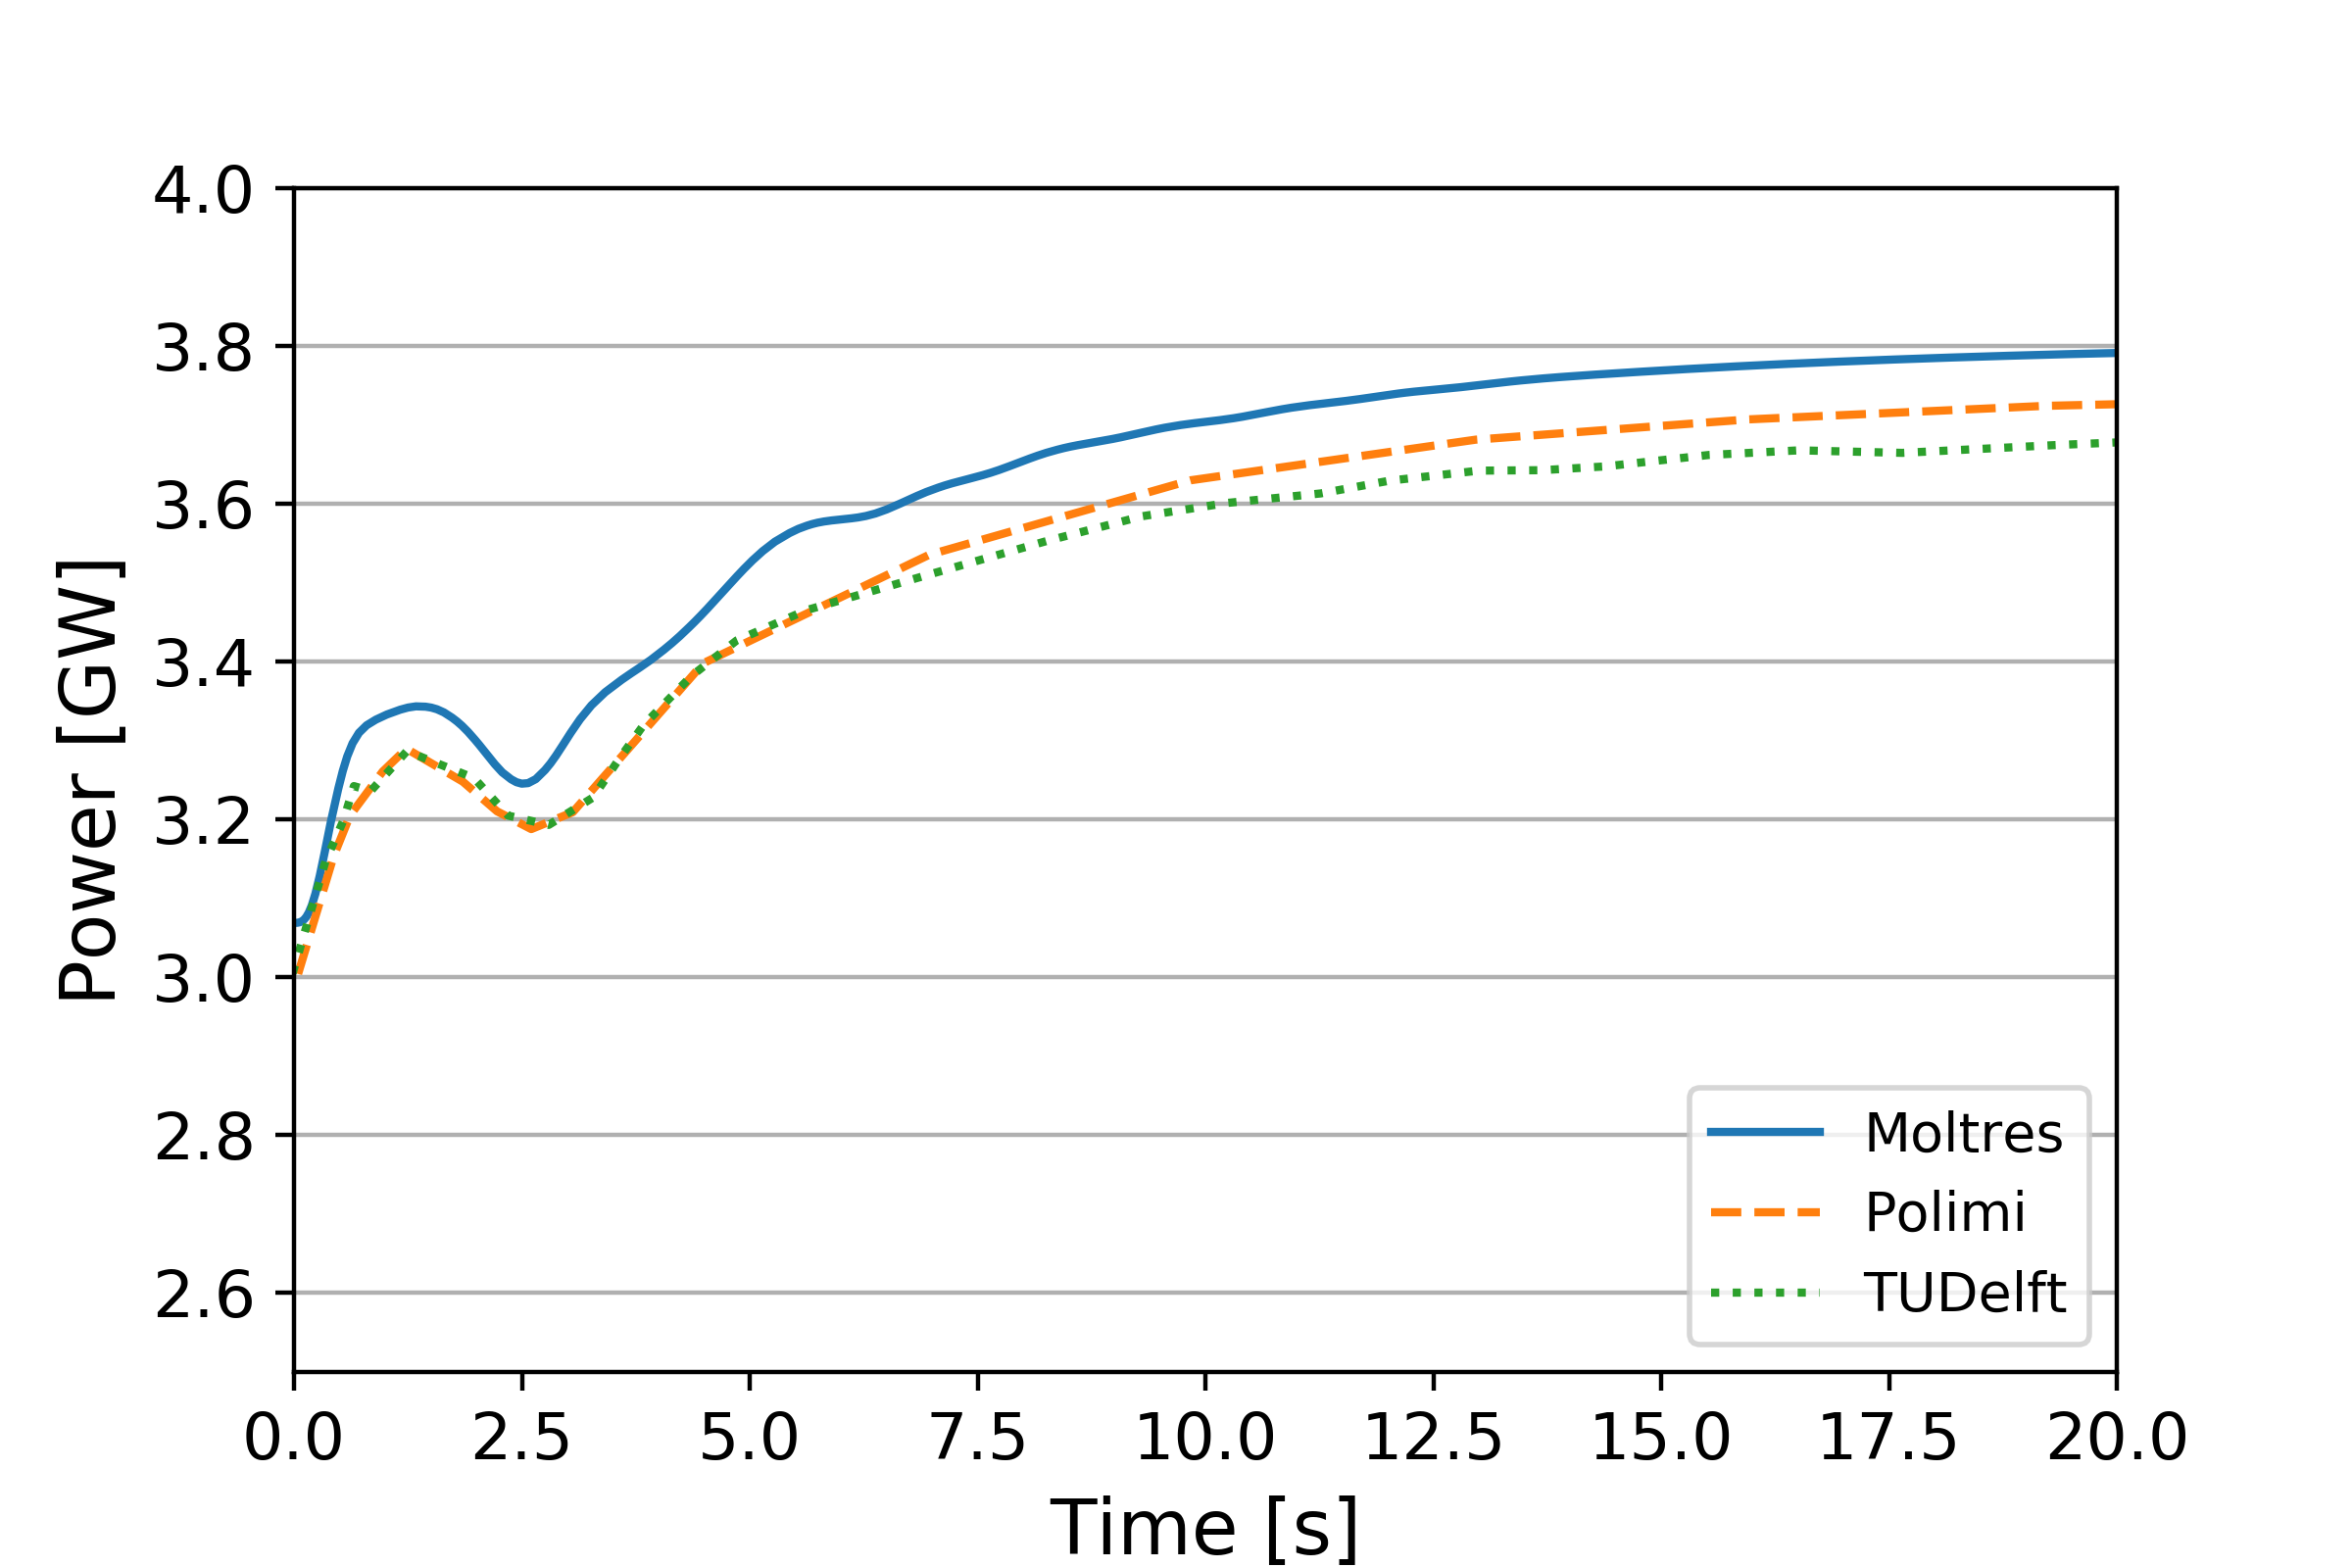
\includegraphics[width=\textwidth]{po-heat-short}
    \end{subfigure}
    \hfill
    \begin{subfigure}[t]{.485\textwidth}
        \centering
        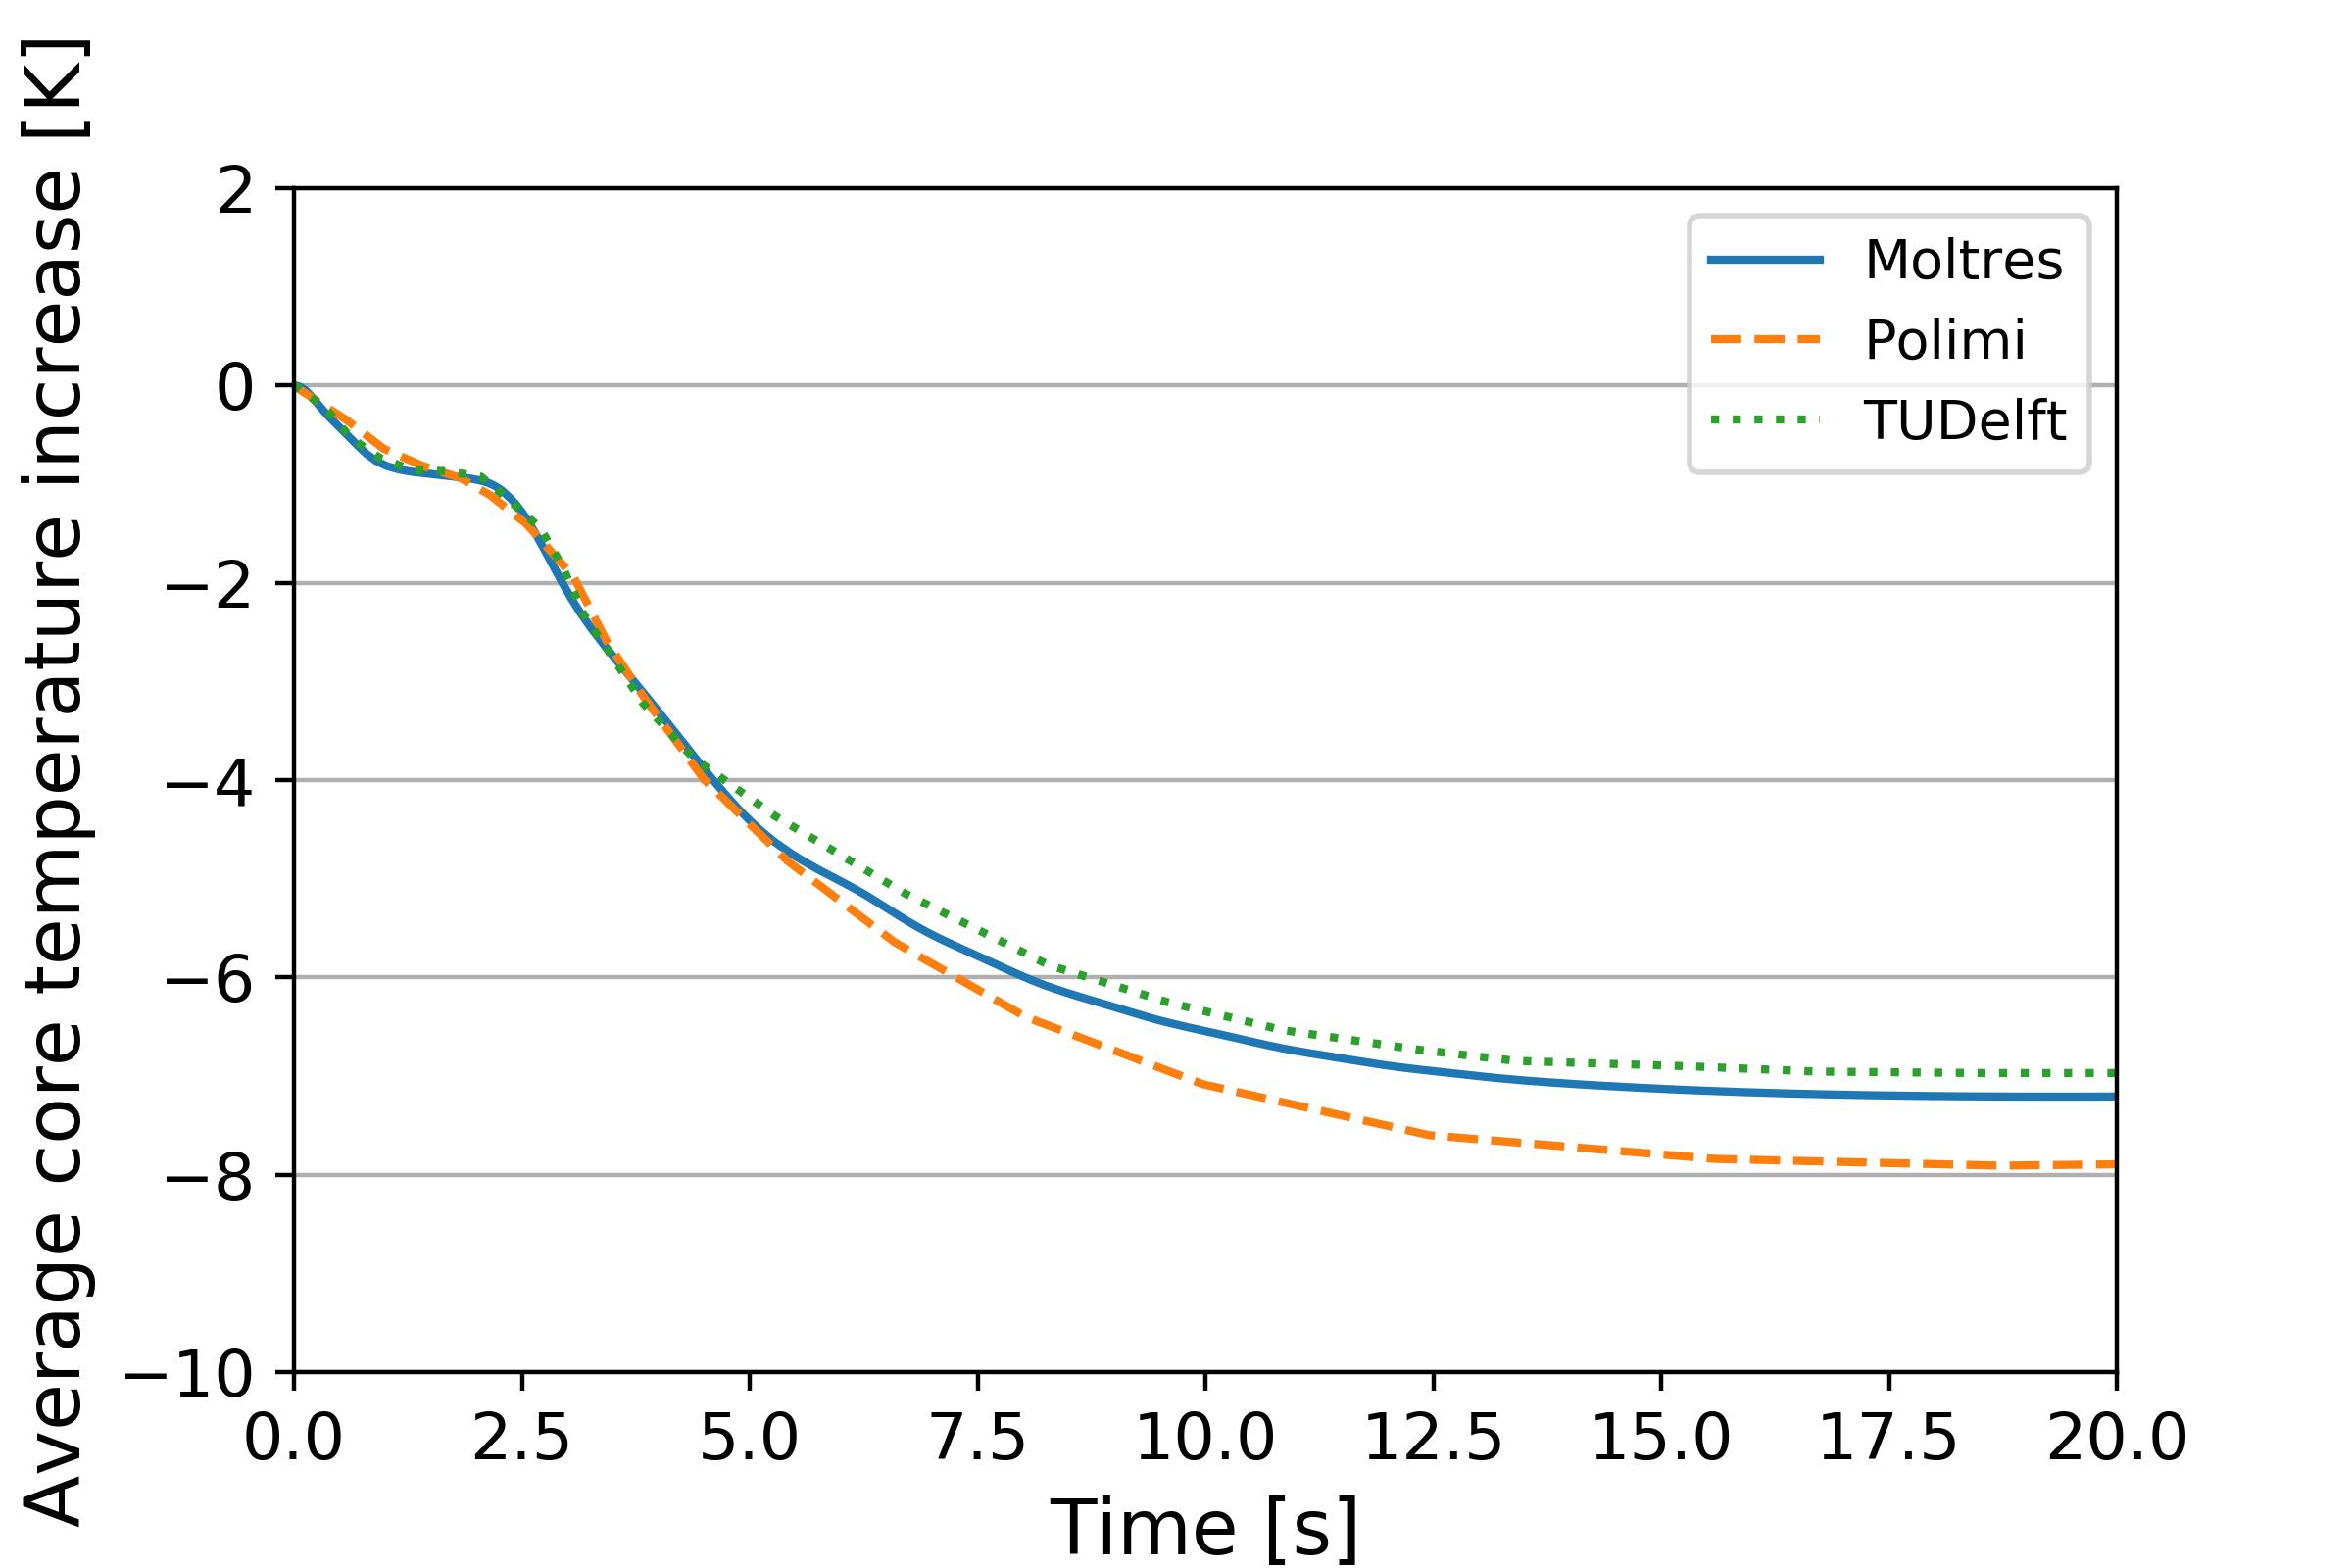
\includegraphics[width=\textwidth]{po-temp-short}
    \end{subfigure}
    \caption{The first 20 s of the power output and average core temperature
    increase during an unprotected pump overspeed transient.}
    \label{fig:poshort}
\end{figure}

The results show excellent agreement with the Polimi and TUDelft models. The
average core temperature increase in particular reproduces the Polimi and   
TUDelft results very well and the curve falls between the other two curves.
The power output is higher because the Moltres \gls{MSFR} model has a
stronger negative temperature coefficient than the other two models. 
